\documentclass{article}

\usepackage{comment}
\includecomment{vfull}
\excludecomment{vcat}
%\includecomment{vdraft}



\usepackage[margin=1in]{geometry}
\usepackage{mathtools} %also loads amsmath
\usepackage{amssymb, bbm}

\usepackage[backend=biber,
	style=alphabetic,
	%	citestyle=authoryear,
	natbib=true,
	url=true, 
	doi=true]{biblatex}

%\usepackage{blkarray} % for matrices with labels
\usepackage{microtype}
\usepackage{relsize}
\usepackage{environ}% http://ctan.org/pkg/environ; for capturing body as a parameter for idxmats
\usepackage{tikz}
	\usetikzlibrary{positioning,fit,calc, decorations, arrows, shapes, shapes.geometric}
	\usetikzlibrary{cd}
	
	\pgfdeclaredecoration{arrows}{draw}{
		\state{draw}[width=\pgfdecoratedinputsegmentlength]{%
			\path [every arrow subpath/.try] \pgfextra{%
				\pgfpathmoveto{\pgfpointdecoratedinputsegmentfirst}%
				\pgfpathlineto{\pgfpointdecoratedinputsegmentlast}%
			};
	}}
	%%%%%%%%%%%%
	\tikzset{center base/.style={baseline={([yshift=-.8ex]current bounding box.center)}}}
	
	\tikzset{dpadded/.style={rounded corners=2, inner sep=0.9em, draw, outer sep=0.4em, fill=gray, fill opacity=0.08, text opacity=1}}
	\tikzset{active/.style={fill=blue, fill opacity=0.1}}
	\tikzset{square/.style={regular polygon,regular polygon sides=4, rounded corners = 0}}
	\tikzset{octagon/.style={regular polygon,regular polygon sides=8, rounded corners = 0}}
	
	
	\tikzset{alternative/.style args={#1|#2|#3}{name=#1, circle, fill, inner sep=1pt,label={[name={lab-#1},gray!30!black]#3:\scriptsize #2}} }
	
	
	\tikzset{bpt/.style args={#1|#2}{alternative={#1|#2|above}} }
	\tikzset{tpt/.style args={#1|#2}{alternative={#1|#2|below}} }
	\tikzset{lpt/.style args={#1|#2}{alternative={#1|#2|left}} }
	\tikzset{rpt/.style args={#1|#2}{alternative={#1|#2|right}} }
	\tikzset{pt/.style args={#1}{alternative={#1|#1|above}} }
	

	\tikzset{mpt/.style args={#1|#2}{name=#1, circle, fill, inner sep=1pt,label={[name={lab-#1},gray]\scriptsize #2}} }
	\tikzset{pt/.style args={#1}{name=#1, circle, fill, inner sep=1pt,label={[name={lab-#1},gray]\scriptsize #1}} }
	
		
		 %\foreach \x in {#1}{(\x) (lab-\x) } 
		 
	\tikzset{Dom/.style args={#1 (#2) around #3}{dpadded, name=#2, label={[name={lab-#2},align=center] #1}, fit={ #3 } }}
	\tikzset{bDom/.style args={#1 (#2) around #3}{dpadded, name=#2, label={[name={lab-#2},align=center]below:#1}, fit={ #3 } }}
	\tikzset{arr/.style={draw, ->, thick, shorten <=3pt, shorten >=3pt}}
	\tikzset{archain/.style args={#1}{arr, every arrow subpath/.style={draw,arr, #1}, decoration=arrows, decorate}}
	%\tikzset{every label/.append style={text=red, font=\scriptsize}}
	\tikzset{dpad/.style args={#1}{every matrix/.append style={nodes={dpadded, #1}}}}
	\tikzset{light pad/.style={outer sep=0.2em, inner sep=0.5em, draw=gray!50}}
	
	
	\newcommand\cmergearr[4]{
		\draw[arr,-] (#1) -- (#4) -- (#2);
		\draw[arr, shorten <=0] (#4) -- (#3);
	}
	\newcommand\mergearr[3]{
		\coordinate (center-#1#2#3) at (barycentric cs:#1=1,#2=1,#3=1.2);
		\cmergearr{#1}{#2}{#3}{center-#1#2#3}
	}

\NewEnviron{ctikzpicture}{\begin{center}\expandafter\begin{tikzpicture}\BODY\end{tikzpicture}\end{center}}
%\newenvironment{ctikzpicture}
%	{\begin{center}\begin{tikzpicture}}
%	{\end{tikzpicture}\end{center}}

\usepackage{color}
\definecolor{deepgreen}{rgb}{0,0.5,0}

\usepackage[colorlinks=true, citecolor=deepgreen]{hyperref}


\setlength{\skip\footins}{1cm}
\setlength{\footnotesep}{0.4cm}


\usepackage{stmaryrd}
\usepackage{trimclip}

\makeatletter
\DeclareRobustCommand{\shortto}{%
	\mathrel{\mathpalette\short@to\relax}%
}

\newcommand{\short@to}[2]{%
	\mkern2mu
	\clipbox{{.5\width} 0 0 0}{$\m@th#1\vphantom{+}{\shortrightarrow}$}%
}
\makeatother

\usepackage{parskip}
\usepackage{amsthm, thmtools}
\usepackage{
	nameref,%\nameref
	hyperref,%\autoref
	% n.b. \Autoref is defined by thmtools
	cleveref,% \cref
	% n.b. cleveref after! hyperref
}

\hypersetup{colorlinks=true, linkcolor=blue, urlcolor=magenta}

\begingroup
\makeatletter
\@for\theoremstyle:=definition,remark,plain\do{%
	\expandafter\g@addto@macro\csname th@\theoremstyle\endcsname{%
		\addtolength\thm@preskip\parskip
	}%
}
\endgroup
\makeatother

\theoremstyle{plain}
\newtheorem{theorem}{Theorem}[section]
\newtheorem{coro}{Corollary}[theorem]
\newtheorem{prop}[theorem]{Proposition}
\newtheorem{lemma}[theorem]{Lemma}
\newtheorem{fact}[theorem]{Fact}
\newtheorem{conj}[theorem]{Conjecture}

\theoremstyle{definition}
\newtheorem{defn}{Definition}[section]
\newtheorem*{defn*}{Definition}
\newtheorem{examplex}{Example}[section]
\newenvironment{example}
	{\pushQED{\qed}\renewcommand{\qedsymbol}{$\triangle$}\examplex}
	{\popQED\endexamplex\vspace{-1em}\rule{1cm}{0.7pt}\vspace{0.5em}}

\theoremstyle{remark}
\newtheorem*{remark}{Remark}

\usepackage{xstring}
\usepackage{enumitem}

\DeclarePairedDelimiterX{\infdivx}[2]{(}{)}{%
	#1\;\delimsize\|\;#2%
}
\newcommand{\kldiv}{D_\mathrm{KL}\infdivx}
%\DeclarePairedDelimiter{\norm}{\lVert}{\rVert}

%\newcommand\duplicat[1]{\gdef\mylist{}\foreach \x in {#1}{\xdef\mylist{\mylist (\x) (lab-\x) }}\mylist} %% this doesn't work :((
\newcommand\lab[1]{(#1)(lab-#1)}


\newcommand{\CI}{\mathrel{\perp\mspace{-10mu}\perp}}
\newcommand\E{{\mathbb E}}


\newcommand{\todo}[1]{{\color{red}\large\textbf{[}{\normalsize\texttt{todo:} \itshape#1}\textbf{]}}}
\newcommand{\note}[1]{{\color{blue}\large\textbf{[}{\normalsize\texttt{note:} \itshape#1}\textbf{]}}}

\newcommand\geqc{\succcurlyeq}
\newcommand\leqc{\preccurlyeq}
\newcommand\mat[1]{\mathbf #1}
\newcommand{\indi}[1]{\mathbbm{1}_{\left[\vphantom{\big[}#1 \vphantom{\big]}\right]}}
\newcommand\m[1]{\mathbf m_{\mathsf #1}}
\def\cpm#1(#2|#3){\mathbf #1 \left[ #2 \middle|#3\right]}


\newcommand\recall[1]{\expandarg\cref{#1}:\vspace{-1em} \begingroup\small\color{gray!80!black}\begin{quotation} \expandafter\csname #1\endcsname* \end{quotation}\endgroup }

%OMG THIS WORKS

\def\wrapwith#1[#2;#3]{
	\expandafter#2{\expandarg\StrBefore{#1}{,}}
	\expandarg\StrBehind{#1}{,}[\tmp] 
	\xdef\tmp{\expandafter\unexpanded\expandafter{\tmp}}
	#3
	\expandarg\IfSubStr{\tmp}{,}{\wrapwith{\tmp}[#2;{#3}]}{ \expandafter#2{\tmp} }
}
\def\hwrapcells#1[#2]{\wrapwith#1[#2;&]}
\def\vwrapcells#1[#2]{\wrapwith#1[#2;\\]}



\newsavebox{\idxmatsavebox}
\def\makeinvisibleidxstyle#1#2{\phantom{\hbox{#1#2}}}
\newenvironment{idxmatphant}[4][\footnotesize\color{gray}\text]{%
	\def\idxstyle{#1}
	\def\colitems{#3}
	\def\rowitems{#2}
	\def\phantitems{#4}
	\begin{lrbox}{\idxmatsavebox}$
	\begin{matrix}  \begin{matrix} \hwrapcells{\colitems}[\idxstyle]  \end{matrix} \\[0.1em]
		\left[ 
		\begin{matrix}
			\hwrapcells{\phantitems}[\expandafter\makeinvisibleidxstyle\idxstyle]  \\[-1em]
	}{
		\end{matrix}\right]		&\hspace{-0.5em}\begin{matrix*}[l] \vwrapcells{\rowitems}[\idxstyle] \end{matrix*}
	\end{matrix}
	$\end{lrbox}
	\raisebox{0.75em}{\usebox\idxmatsavebox}
%	\vspace{-0.5em}
}

\newenvironment{idxmat}[3][\footnotesize\color{gray}\text]
	{\begingroup\idxmatphant[#1]{#2}{#3}{#3}}
	{\endidxmatphant\endgroup}

\newenvironment{sqidxmat}[2][\footnotesize\color{gray}\text]
	{\begingroup\idxmat[#1]{#2}{#2}}
	{\endidxmat\endgroup}
	
	
%%%%%%%%%%%%
% better alignment for cases
\makeatletter
\renewenvironment{cases}[1][l]{\matrix@check\cases\env@cases{#1}}{\endarray\right.}
\def\env@cases#1{%
	\let\@ifnextchar\new@ifnextchar
	\left\lbrace\def\arraystretch{1.2}%
	\array{@{}#1@{\quad}l@{}}}
\makeatother
\usetikzlibrary{external}
\tikzexternalize[prefix=tikz/]  % activate!

\AtBeginEnvironment{tikzcd}{\tikzexternaldisable} %... except careful of tikzcd...
\AtEndEnvironment{tikzcd}{\tikzexternalenable}


\usepackage[nointegrals]{ wasysym }

\addbibresource{../refs.bib}
\addbibresource{../maths.bib}


% symbols for genders, hour glass.
\newcommand{\mfem}{\mathclap\female\male}
\newsavebox{\hourglassbox}
\savebox{\hourglassbox}{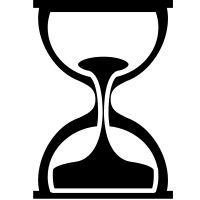
\includegraphics[height=.8em]{hourglass.png}}
\newcommand\hourglass{\usebox{\hourglassbox}}


%flags for full vs short vs draft version. 
%\def\vshort{}
%\def\vfull{ \begin{verfull} }
%\newcommand{\vdraft}{}

\title{Merged: Dynamic Beliefs and Preferences}
\author{Oliver Richardson  \texttt{oli@cs.cornell.edu}}


\begin{document}
	\maketitle
	
	\section*{A Quick Overview}
	In some sense, the goal of this project is to provide a compelling picture of preference revision --- but in doing so, we will paint a very different, generalized picture of decision theory. 
	
	The core representation we suggest, the marginal constraint graph, is more flexible than the standard ones, as agents need not always have a perfectly consistent picture of reality, intermediate representations have meanings, and we can capture phenomena such as learning preferences from data and revising them in various places. In special cases, we recover standard results, including expected utility calculations, belief updating by conditioning.
	
	We can roughly separate the work into two pieces:
	\begin{enumerate}%[nosep]
		\item Representation: the sufficiency of our new representation as a unification of existing results. In particular, we think of an agent's values as distributed across a network of concepts, whose nodes are preferences on small sets of alternatives, and whose edges are beliefs about the impact of one variable on another.
		\item Dynamics: A formulation of how to revise the representation in light of new information or additional computation. We will show how can be dealt with through inconsistency, illustrate some options for regularization, and ultimately factor out these as general meta-preferences. 
	\end{enumerate}

	\tableofcontents
	\clearpage
	\part{Motivations}
%	This work an be motivated in many different ways; I imagine the most compelling one to depend on who you are and what you already care about. In any individual paper I plan to only include one of these, but until the audience has been narrowed, I want to keep all of them around. %to remind myself which directions I want to push, and to record selling points outside of the best publishing path.

	\begin{ctikzpicture}
		\node[ellipse,draw,align=center] (R) at (4,-3) {World\\ Representation};
		\node[ellipse,draw] (B) at (3,1) {Beliefs};
		\node[ellipse,draw] (V) at (3,-1) {Values};
		\node[ellipse,draw] (A) at (5.5,0) {Actions};
		
		\draw[arr,-] (B) -- (4,0) -- (V);
		\draw[arr, shorten <=0] (4,0) -- (A);
 	\end{ctikzpicture}


	\section{Issues with Standard Issue Decision Theory}
	\subsection{Some Reasons not to Calculate Expected Utility}
	
	\begin{enumerate}
		\item \textbf{No utility function}. Maybe your preferences are not representable in this way --- maybe they violate the vNM axioms, or you just don't have anything that resembles an ordered set. Maybe your intrinsic utility is stochastic.
		
		\item \textbf{No complete prior.} It is possible that you're not a Bayesian, and don't have (access to) a probability distribution on all salient features of your world\footnote{In fact, once we add enough representational complexity to our world, this is impossible to have; see section \ref{sec:impossible-prior}}.  
		%		Of course, if you accept Savage's axioms, then you act as though you have both a probability distribution over states and a utility function
		
		\item \textbf{Thinking takes time.} (this constrains the complexity of your utility and probability information, or at least requires them to be in a form that admits fast computations)
		
		\item \textbf{Internal Actions.} In addition to the external actions, there are also invisible mental ones: nobody has complete control over what they do in all respects at all times. Emotionally preparing yourself to talk to your boss, warming up your fingers to play piano, and intentionally committing a phone number to memory are all examples of mental actions, which are rarely modeled. More generally, for any interface with the world that a model prescribes, there will be extra 
		
		%you may not know exactly what it is you have to do in orde to 
		\item \textbf{Different world representation.} 
		%			You have a distorted perception of the world. 
		Models, both in probabalistic reasoning and decision theory, usually start by defining the set of possible states of the system. For a modal logician, this is the underlying set of a Kripke structure; for probability theorists, it's a set of outcomes.This is fine if agents are aware of the structure you've set up, but simply don't know what world they're in --- but nothing precludes them from conceptualizing things in entirely different terms. 
		
		When the agent fails to obey expected utility for this reason, there are three ways to assign blame: it could be the agent's fault for not truly understanding what is possible, the modeler's fault for failing to capture the the agent's picture of the world.
		
		
		
		\item \textbf{Things Change over Time.}
	\end{enumerate}	
	
	Despite the fact that there has been work backing off of each of these assumptions, utility maximization is still ubiquitous (and taken for granted) in most primary applications, including consumption models and the construction of artificial agents. In section \ref{sec:optimization-bad} I argue that this is the source of some cultural problems. But part of the reason that many of the other techniques has not gained traction is that none is as clean and as useful as expected utility maximization, and to the best of my knowledge people try to isolate and tackle these issues individually. My framework provides a way of representing many of these issues effectively and cleanly, while also reducing to the expected utility computations when none of these issues apply. 
	
	
	\subsection{Fixed World Representation}
	
	The set of things which are even considered possible is contentious enough that we don't want to build it (and actually the correct one) canonically into an agent's picture of the world. In some sense only the current world is possible, as far as anyone can be sure. Moreover, no matter how you chose to represent the world, an agent's picture of what's possible can change over time, which means the modeler needs to write down beforehand everything that could possibly happen. We talk more about this in section \ref{sec:cat-worlds}
	
	\subsubsection{World Explosion} \label{sec:world-explosion}
	
	\section{The Big Picture: Why This is Important}
	\begin{enumerate}
		\item Subjective representations of the world
		\item Joint dynamics
		\item 
	\end{enumerate}

	\subsection{Fixing the Ethos of Agency}
	The distinction between the things that you care about (e.g., utilities, goals, preferences, objectives), and the tools you have for understanding and affecting the world (e.g., beliefs, reasons, plans, optimization, inference) plays a large role in technical accounts of agency%
	\footnote{Beliefs should be considered optimization power: they you believe that action $A$ will have effect 1, an action $B$ will have effect 2, and a preference between the 1 and 2}.
	Generally the two are considered separately, and also people tend to fix preferences%
	\footnote{In the context of optimization, this corresponds to the practice of writing down an objective and finding extrema; in the context of decision theory, it is finding the best actions to satisfy some preferences}. 
	%
	This is nice because the fixed preferences provide a clean way to evaluate the quality of decisions, and criteria for success are a very important part of science. It is clear why modeling things in this way caught on so quickly and durably --- it is simple, prescribes tractable computations, is expressive enough to capture any behavior over fixed time periods, if you make modeling choices in the right ways. 
	
	This heavy dependence on modeling assumptions is an underappreciated shortcoming, and freedom to chose the representation gives modelers a lot of power to over-fit to their desired outcomes. 
	
	
	In real life, human preferences and beliefs often depend on one another, and in more complex settings the line is much more blurred:
	%	Subjectively, though it is hard to imagine having one without the other, and it seems like there might be G\"odelian knots if you take the separation seriously enough --- 
	\begin{itemize}
		\item When you play a video game, are you trying just so you can win? If so, why do you care about winning? Decision theorists often take this as primitive, but it can also be considered in a larger picture, which decision theorists also purport to model. It buys you very little socially, and costs time and money. Or does the process of optimizing for this arbitrary goal itself have value? Does this make entertaining yourself fundamentally irrational?
		%		\item In the process of achieving enlightenment, you go about removing your desires. But it seems like being without desires is in fact a desire--- why where you attempting to do this, anyway? 
		%		\item Similarly,  care about is truth
		\item It is common for humans to have beliefs about preferences: (`I think I like cheese', 'I believe freedom is bad'), and also preferences over beliefs (`Believing true things is good', `I want to know calculus') --- but the clear separation in standard decision theory makes this difficult to understand. 
		
		These can be nested quite deeply without anyone thinking too hard: If I ask if you like cheddar, you now believe that I want to know whether you like cheese --- note that this is a belief about a desire for a piece of knowledge about a preference, spanning multiple people.
		
		\item On a small scale, we think of a loss function as an optimization objective, and the algorithm (say, stochastic gradient descent) as optimization power. One can use both of these together to form a neural network, which is thought of as being just a tool, with no
		
		\item Complete agents can be used in either way: people, who have desires and experience emotions, can be used as optimization power with an external objective (e.g., hiring employees), but can also as the ultimate source of value (e.g., running an organization because it will help people)
	\end{itemize}
	This is an argument against the orthogonality hypothesis \cite{orthogonality}, and similar lines of thought. It seems clear that if we could combine any picture of truth, with any model of value, and any optimization procedure, which look remotely like those that humans have, the interactions between them would certainly be woven together, and their dynamics would be intertwined.
		
	%%
	{\color{green!30!black}This is why we model the dynamics of beliefs and preferences together, and why in some cases we will be able to represent a belief as a preference or vice versa%
		\footnote{the categorical interpretation, where each node is a category, the big graph forms a 2-category, and beliefs are value-preserving functors, supports the observation that the distinction between preferences and beliefs isn't a fundamental feature the objects themselves but rather how they're used--- here the arrow category here gives us preferences over beliefs. Similarly, quotient objects represented as arrows, just as utilities can be identified with beliefs about utilities.}.
	The way we've laid things out, the interaction between the two resembles a duality.
	}
	
	\subsection{Better Models of Humans, whose Preferences Change}
	When you're born you have no conception of what foods or professions or ideals are good; all you have is your own evolutionarily programmed pleasure and pain. Not only does this feeling get more sophisticated in a way that seems to depend on the environment, but also later on in life, people willingly sacrifice their experiential pleasure for other things they care about. All of this stands even if we didn't see change in the more obvious toy cases: foods, activities, and luxury goods. Such changes do in fact occur, and do not detract from a person's ability to be conceptualized as a coherent agent; often they contribute to a person's character instead.
	
	The standard models do not account for any of this, and for many good reasons --- but dynamic preferences are necessary to capture a great deal of human behavior, and are much more important in a world where value is informational and changes quickly. Things like memes, fashion, games, conversations, lofty ideals, and art---things that standard economic theory has had a lot of difficulty ascribing value to---certainly play a bigger economic role than they have in the past, and arguably move faster as well.
	%is learning a new piece of information something that has value?
	
	%there is some overlap between conditioned preferences and dynamic preferences.
	\subsubsection{}
	{\color{green!30!black}This is why we model changes in preferences, and acquisition from only a very limited set of base values. We have some reasons to suspect that in most cases preferences generated this way will be similar, which if true would (1) provide an additional explanation (beyond empathy and genetics) for why humans end up sharing a lot of values, and (2) allay some concerns about misaligned AIs that are constructed in this way}
	
	\subsection{Computational Tractability}
	
	The standard picture of decision theory requires keeping around preferences and beliefs about all possible things that are relevant to any decisions you make. \todo{Is there an edit here to be made about small vs large worlds?} To fully describe a general agent's values, then, you need to specify a preference ordering over all possible histories of settings of observable features. This is wildly intractable, and also annoyingly depends on what ``possible'' means, which is part of the agent's internal beliefs\footnote{Or alternatively, if you're going to do the work beforehand as a modeler, has to change when humanity discovers new features of the universe}. This is why people in practice restrict the scope of an agent to only a few modeler-chosen variables, assume that they only encounter one kind of decision, specify objectives in a compressed syntactic form.
	
	But even these more tractable restricted approximations we use do not degrade gracefully: in order to make any decisions at all you have to do expected utility calculations (which could be very expensive depending on how clear the impact of your decision on the world is), and there's certainly no clear way of making use of partial computations under time pressure.
	
	{\color{green!30!black} By keeping parts of preferences around in many different forms, attached to different contexts, not only can we immediately re-use them for recent decisions we've made in a pinch, but also reduce the complexity of adding new nodes. This is because we can split the computation into meaningful chunks (one for each preference domain (node) we can connect a decision to).}
	
	\todo{mention related work on tractability: BN's, Markov Networks, Markov Networks}
	
	\subsection{The Value Of Inconsistency.}	
	
	%% bad, unclear paragraph
	There are still many tasks human-coded expert systems excel at, which are difficult for trained statistical systems. However, they are slowly losing their ground due to a debilitating shared flaw: any input that the designer has not anticipated causes the entire calculation to be wrong in un-salvageable ways. From the perspective of the expert system, though, there is nothing wrong. 
	
	The program is specified by \emph{behavior},  It's coded without an outside view of the explicit purpose: there's no possibility that the designer was \textit{wrong} in the algorithm specification, and there's no reasonable inference to make instead even we acknowledged it was possible she was.
	
	\textbf{The only way you can know if you're wrong is if there is enough redundancy to highlight inconsistency.}
	
	Incorporating probabilities and specifying objectives instead of algorithms has helped this problem enormously: by using a ton of redundant, noisy, examples of the algorithm working correctly, we can be reasonably resistant to malformed input. Unfortunately, these systems are not perfect either: they are often biased and sometimes cheat. We face a different kind of brittleness here: what if we forget about a second order effect and slightly mis-specify an objective function? What if we run it on a different input distribution? ML systems won't crash, but they will confidently display  wrong answers. The system doesn't think there's any possibility that its \textit{objective is wrong}, and even if it acknowledged this possibility, it's not clear there's anything to be done at this point.
	
	{\color{green!30!black}In analogy to the solution that statistical ML provided to the problem of brittle classical AI, the solution would seem to be a noisy, redundant encoding of the objective function in conjunction with a meta-objective: in our case, consistency. The diffusion of preferences (which we will also refer to as value capture) can also be thought of as a source of uncertainty about your values even if you didn't start with any: if there are multiple objectives consistent with everything you've seen, you acquire a preference for both of them.}
	
	Of course, humans are also often uncertain about their values (and experience value capture) in addition to their beliefs and the appropriate choice of actions.
	%	Agents are allowed to have uncertainty in what they believe
	
	%	nd so the synthetic agents we design, influenced by the standard picture and designed with particular use cases in mind, 
	
	
	
	\subsection*{[Theoretical Unity] Reductions to other theories and algorithms} \todo{Edit this}
	%	There are many different representations of preference theories 
	The generality is a genuine mathematical motivation for this theory: it can be viewed as a number of different things. I will briefly mention some of them that I'm excited about here, and then focus on simple things for the rest of the document.
	\begin{itemize}[nosep]
		\item Our model reduces to standard expected utility calculations in the degenerate case where the agent has preferences over possible histories of worlds, the representation of a world never changes, and the agent is cognitively unbounded
		\item It has a categorical interpretation which has some features I'd like to explore: in particular, meta-preferences seem to be related to higher order structure, a total utility function is like a limit, a total probability function is like a co-limit, preference-preserving beliefs are functorial, and the nodes already form a 2-category, whose objects are themselves enriched flat categories.
		\item There also a natural interpretation of this as an artificial neural network. If the underlying graph is a DAG with one sink, then it is a feed-forward network for calculating expected utility. In most interesting cases, it will have recurrent connections and no special output.
		\item For agents that have priors, the beliefs encoded in this way can be converted to a Baysian Network with a simple transformation
		%		\item If the nodes are all propositions with a preference for truth, and we add some explicit rules for creating and deleting nodes, it becomes an inductive theorem prover.
		\item The preference propagation is a bit like broadcasting on a network (of physical machines) to compute path lengths. This can be done Dijkstra / Distributed Bellman Ford \footnote{depending on whether we take right or left powers of matices} and can be computed by taking iterative powers of a giant matrix over the tropical semi-ring. Funnily enough, this is exactly how you compute the transitive closure of preference matrices on a small scale (except with a different semi-ring), which lends more credibility to the higher order categorical interpretation.
	\end{itemize}
	
	The possibility of bridging these many disparate fields makes the abstraction feel much more universal, and the ability to think about preference change in any of these terms could make it easy to identify analogs of non-trivial facts in other fields.
	
%	These are features that we would like to explain in humans, but needn't necessarily be essential .

%	\section{A Temporal Extension}
%	
%	Many issues with decision theory can be attributed to a failure to account for the passage of time. 
%	One popular example of this is the ubiquitous assumption of cognitive unboundedness: in a static world, where everything is frozen except your own thoughts, you can afford to do decision theory exactly by computing expected utility. You have only one decision to make
%	
%	Still, cognitive boundedness is only one example. When we move to a dynamic setting, most classical results no longer apply, though people often like to pretend that they do. 
%	\begin{enumerate}
%		\item There's no reason to 
%	\end{enumerate}
%	
%	If your beliefs
	
	
%	\section{Better Models of Humans}

	\section{Desiderata}


	%	Currently preferences are thought of as static objects, fixed as part of the structure and identity of an agent, independent of beliefs, complete, and over some fixed domain. This is clearly not at all how human preferences work, and I posit that it's not the right way to think of preference for synthetic agents either.
	
	Perhaps among other things, any model of preference dynamics that is to be used to build synthetic agents which have control over important decisions, should have the following properties: 
	\begin{enumerate}[noitemsep, label=\textbf{D\arabic*}.]
		\item Provide an answer to the `value loading' problem: show how you can learn ``reasonable'' preferences by interacting with the world
		\item Reduce to static models for some parameter settings
		\item Behave reasonably when combined with changes of perspective 
		\item Be resistant to standard challenges to irrationality, such as dutch book arguments
		\item Have weak safety guarantees: an agent should not eagerly adopt preferences which are totally in conflict with its current ones
	\end{enumerate}
	
	%	We might also require that a theory be useful for explaining human behavior. We expect ours to be able to explain:
	Because the view of preferences we adopt here is different from the standard ones in economics (in particular, it lends itself naturally to incorporating boundedness), we have a hope of explaining some behavior which was previously classified irrational, as an optimal in some sense. The following psychological effects lend themselves to explanation:
	\begin{enumerate}[noitemsep]
		\item \textbf{Value Capture.} You really care about $X$ (say, learning math), which is vague and hard to measure, so you come up with some metric $Y$ (say, scores on undergrad math exams). Over time, optimizing for $Y$ will cause you to optimize less effectively for $X$ and assign intrinsic value to $Y$ (getting good exam scores becomes valuable, independent of whether you learn math\footnote{Social signaling plays into this, but this occurs also in cases where people try to hide the signal: constant grade checking, pokemon go addiction, etc.}). Related to Goodhart and Cambell's laws.
		\item \textbf{Framing Effects.} It is well-documented that the style of presentation, even for logically equivalent scenarios, can have a significant impact on a person's choice. But if we formalize these as the same outcome, there's no way for utility-maximizing agent to behave this way.
		\item \textbf{Connoisseur Effects.} Someone who listens to a lot of rap music has more nuanced, complicated preferences on rap music than someone who has not heard as much. Similarly, people work to develop palates for wine, and ``all Indian food tastes the same'' is an insult, indicating a shallow experience with the cuisine. There are two technical aspects: first, additional experiences increase preference complexity.
		
		\item \textbf{Adaptive Preferences.} Even things we find objectionable are normalized over time, and people often change to prefer things they're used to, even if they are initially opposed. This is sometimes thought of as a prioritization of safety, and is maybe best thought of as a thought-saving feature: the things you're used to have gotten you this far already. 
		
		%		\item \textbf{}
		
		\item \textbf{Novelty Effects (anti-adaptive preferences).} 
		
	\end{enumerate}


	\clearpage
	\part{Probabilistic Constraint Graphs}
	The basic tool that we will use to solve these problems is a graphical representation of (a piece of) an agent's mental space, which we call a marginal constraint graph. Throughout this section, we will introduce them from many different perspectives, but They look a bit like Bayesian Networks, but are more general: rather than representing a single distribution, they represent (soft) constraints on distributions. 
	
	\begin{itemize}
		\item If the constraints pick out a single distribution, the PCG is a graphical factorization of that distribution. 
		\item If the PCG is under-constrained, there are many distributions consistent with it. We can use this to emulate weaker notions of uncertainty than probability distributions themselves. However, not all such distributions are equal: some may be simpler than others, or better match the symmetries of the constraints; we use entropy to distinguish between them.
		\item An over-constrained PCG is has internal inconsistencies, the resolution of which drives belief and preference change. Just as in the under-constrained case, not all resolutions are equal: some are more or less constrained 
	\end{itemize}
	
		

	\section{Uncertainty Examples \todo{fold into other sections}}
	\subsection{Coin Tosses}
	\begin{example}
		You're about to flip a coin. The result of this flip is the only thing you're thinking about, but you know nothing about the outcome, other than that it could land heads or tails. This (lack of) knowledge is the single node in an PCG:

		\begin{ctikzpicture}
			\node[bpt={h | $H$}] at (-0.3,0) {};
			\node[bpt={t | $T$}] at (0.3,0) {};
%			\draw[arr,->, thin, red, dashed] (x1) to[bend right=40](x2);
			\node[bDom={Coin (C) around \lab{h}\lab{t}}] {};
		\end{ctikzpicture}
		
		One might think this is vacuous, but in fact this conveys two important things: that the agent is aware of and conceptualizes the coin flip (with the two outcomes), and a total uncertainty about what values they actually take and how they relate to anything else.
	\end{example}

	\begin{example}
		Now you start reasoning about this coin, and decide that the outcome of the flip is determined by some intrinsic feature of the coin: its bias; you'd be willing to assign a probability to the coin flip if you knew the bias. We illustrate this with the following diagram:
				
		\begin{ctikzpicture}
			
			\node[bpt={h | $H$}] at (-0.3,0) {};
			\node[bpt={t | $T$}] at (0.3,0) {};
			%			\draw[arr,->, thin, red, dashed] (x1) to[bend right=40](x2);
			\node[bDom={Coin (C) around \lab{h}\lab{t}}] {};
			
			
			\node[dpadded, left=1 of C] (B) {$\sf Bias$};
			
			
			\draw[arr] (B) -- (C);
		\end{ctikzpicture}
	
		where Bias is some value in $[0,1]$ and the arrow $P$ is given by 
		\[ P : \mathsf{Bias} \to \Delta \{H, T\}, \qquad P(b)  =  \begin{cases}
		 	H & \text{with probability $b$} \\
		 	T & \text{with probability $1-b$}
		\end{cases} \]
		Bias is now an infinite random variable, and functions as a higher-order probability, which has been "internalized" to the picture. Doing this again may seem vacuous, as we have not gained any information about whether the coin will land heads or tails, but once again we get information about what the agent thinks is relevant. Putting this node in the space can make otherwise innocuous changes suddenly meaningful --- for instance, if Bias had only a finite selection of possibilities, a granularity perhaps imposed by the agent's way of representing numbers, then the agent has given themselves information about the coin through arbitrary choices.
	\end{example}


	\begin{example}
		We will take our coin example a bit further. Already in the previous case, the set of biases is consistent with some set of distributions. Suppose that our agent continues to think and realizes they consider some set of distributions over bias possible. Now that they are aware of it, we give it a name ($\sf S$), and put it into the picture:
		
		
		\begin{ctikzpicture}
			
			\node[bpt={h | $H$}] at (-0.3,0) {};
			\node[bpt={t | $T$}] at (0.3,0) {};
			%			\draw[arr,->, thin, red, dashed] (x1) to[bend right=40](x2);
			\node[Dom={Coin (C) around \lab{h}\lab{t}}] {};
			
			
			\node[dpadded, left=1 of C] (B) {Bias};
			\node[dpadded, left=1 of B] (S) {$\sf S$};
			
			
			\draw[archain] (S) -- node[above]{$q$} (B) -- (C);
		\end{ctikzpicture}
		
		The arrow $q$ represents the conditional distribution $\mu_s$ on Bias, for $s \in S$. This example illustrates that not only can these PCGs represent sets of distributions with some external interpretation, but this can also be internalized to the PCG itself, and so the kind of inference that can be done externally with lower probabilities, for instance, can be done just by the the prescribed decision theory. 
		
		For example, if $S = \{ \mu_B : \mu_B(H) > 0.5\}$, i.e., you are certain that the probability of heads is at least 0.5 (maybe you know the company which makes it, which only weights the head side, but can do any amount), and you are trying to decide whether to bet that the coin lands heads or tails, you now have the following picture:
	
		\begin{ctikzpicture}
			
			\node[bpt={h | $H$}] at (-0.3,0) {};
			\node[bpt={t | $T$}] at (0.3,0) {};
			%			\draw[arr,->, thin, red, dashed] (x1) to[bend right=40](x2);
			\node[Dom={Coin (C) around \lab{h}\lab{t}}] {};
			
			
			\node[dpadded, left=1 of C] (B) {Bias};
			\node[dpadded, left=1 of B] (S) {$\sf S$};
			\node[dpadded, below=0.8 of C] (Bet) {Bet};
			\node[dpadded, above right=0.4 and 1.9 of Bet.center] (money) {\$};
			
			
			\draw[archain] (S) -- node[above]{$q$} (B) -- (C);
			\mergearr{Bet}{C}{money};
		\end{ctikzpicture}
	
		From this, even though I have no prior on $S$, I know that no matter what distribution on bias is actualized, an even bet for heads nets more money than an even bet for tails. 
	\end{example}

	\begin{example}
		Finally, we can also add weights, which we can use to reason about higher order probability, although we need to be careful about normalization and our arrows will either need to be interpreted as non-standard measures, or we have to make some extra assumptions in the general case. Intuitively, the picture looks like this:
		
		\begin{ctikzpicture}

			
			\node[bpt={h | $H$}] at (-0.3,0) {};
			\node[bpt={t | $T$}] at (0.3,0) {};
			%			\draw[arr,->, thin, red, dashed] (x1) to[bend right=40](x2);
			\node[Dom={Coin (C) around \lab{h}\lab{t}}] {};
			
			
			\node[dpadded, left=1 of C] (B) {Bias};
			\node[dpadded, left=1 of B] (S) {$\sf S$};
			\node[dpadded, left=1 of S] (1) {$\sf 1$};
			
			\draw[archain] (1) --node[above]{$p$} (S) -- node[above]{$q$} (B) --node[above]{$r$} (C);
		\end{ctikzpicture}
	 	Now we finally have grounded the chain so that it has the unique node $\sf 1$ as a root of a tree, and so by Proposition \ref{prop:prob-eq}, there is exactly one distribution consistent with it. We can see that the higher order probability is still represented, and modifications to the arrows which represent more abstract concepts do change the rest of the problem setup --- but at the end, we can use composition (which here is acting as the bind of our probability monad) to squash all of the information a probability.
	\end{example}

	
%	\subsection{Unknown Number of Balls}
	\subsection{Pardoned Prisoner}
	
	
	\begin{example}
		We take this example as well from the Reasoning about Uncertainty book. Suppose there are three prisoners, $A$, $B$, and $C$. One of them has been chosen at random to be pardoned. Prisoner $A$ asks the executioner which of the other two was executed. Just before she gets her answer, the agent's PCG looks like this:
		
		\begin{ctikzpicture}
			\node[dpadded] (1) at ( -2,0) {$\sf 1$};
			
			\node[rpt={a | $A$}] at (0,0.6) {};
			\node[rpt={b | $B$}] at (0,0) {};
			\node[rpt={c | $C$}] at (0,-0.6) {};
			
			%			\draw[arr,->, thin, red, dashed] (x1) to[bend right=40](x2);
			\node[bDom={{Pardoned \\ Prisoner} (PP) around \lab{a}\lab{c}}] {};
			
			\node[rpt={b2 | $B$}] at (3, 0.6) {};
			\node[rpt={c2 | $C$}] at (3,-0) {};
			\node[bDom={{Revealed \\ Condemned \\ Prisoner} (CP) around \lab{b2}\lab{c2}}] {};
			
			\draw[archain] (1) -- (PP) -- (CP);
		\end{ctikzpicture}
	
		Note that in order to tie together the two nodes with an arrow, we need to either know the probability of each prisoner being pardoned for each choice of revealed condemned prisoner, or more naturally, the probability that the executioner reveals each prisoner, given the identity of the pardoned one --- that is, we need to model the protocol of the executioner. If we assume the executioner is truthful, we still need to know what happens when $A$ was the pardoned prisoner and the executioner has a choice. Suppose that in this case, $B$ is always revealed. This results, through composition, in a prior distribution over the revealed prisoner, with $\frac{2}{3}$ on $B$ and $\frac{1}{3}$ on $C$.
		
		
		Once we make our observation, we get a new arrow; suppose we hear that $B$ was revealed.
		
		\begin{ctikzpicture}
			\node[dpadded] (1) at ( -2,2) {$\sf 1$};
			
			\node[rpt={a | $A$}] at (0,0.6) {};
			\node[rpt={b | $B$}] at (0,0) {};
			\node[rpt={c | $C$}] at (0,-0.6) {};
			
			%			\draw[arr,->, thin, red, dashed] (x1) to[bend right=40](x2);
			\node[bDom={{Pardoned \\ Prisoner} (PP) around \lab{a}\lab{c}}] {};
			
			\node[rpt={b2 | $B$}] at (3, 0.6) {};
			\node[rpt={c2 | $C$}] at (3,-0) {};
			\node[bDom={{Revealed \\ Condemned \\ Prisoner} (CP) around \lab{b2}\lab{c2}}] {};
			
			\draw[archain] (1) -- (PP) -- (CP);
			\draw[arr, dashed] (1) to[bend left=10] (CP);
		\end{ctikzpicture}
		There is now an inconsistency: the two paths from 1 give different distributions on the revealed prisoner. There are many ways to ameliorate this:
		\begin{enumerate}[nosep]
			\item The agent can ignore what the executioner told her, because it conflicts with your a-priori distribution on the probability of what the executioner would say
			\item The agent can revise their view of the executioner's protocol upon hearing $B$, and now believe that the executioner would have told her this no matter who was pardoned.
			\item The agent can change their belief about how likely each prisoner is to have been pardoned. In this case, she can conclude that her chances of dying are now 1 in 2. Of course, if the executioner had said $C$, she would have had to conclude she was guaranteed to die.
		\end{enumerate}		
	\end{example}

	\begin{example}[Prisoners and subdistributions]
		Maybe we actually do not know the guard's protocol. We can still interpret the arrow as a sub-Markov transition / sub-stochastic matrix, where now we do not know what happens when $A$ is the pardoned prisoner. In this case, we still can compose the arrows, and obtain a sub-distribution $\Pr_*(B) = \frac{1}{3}$, $\Pr_*(C) = \frac{1}{3}$. Upon hearing the name of the revealed prisoner, we cannot update, and still have the same sub-distribution. 
	\end{example}

	
	
	
	\section{Definitions and Semantics}
	\begin{defn*}[PCG, semi-formal]\label{def:pcg-semiformal}
		A marginal constraint graph $(\cal N, L)$ is a collection of variables $\cal N$, attached to each of which is some preference information: (this could be an order, utility, pairwise utility matrix, a supremum function), plus a collection of probabilistic links $\cal L$ between some (but not necessarily all) pairs of them, where $L: A\to B \in \cal L$ is a (sub) Markov kernel $A \to \Delta [B \cup \{\bullet\}]$\footnote{The additional ``phantom element'' $\bullet$ absorbs probability density that we don't want to equivocate on, allowing our model to capture partial families of conditional probabilities, by extension things like implication, and giving agents more tools to avoid inconsistency. This has the effect of making our links substochatic matrices/kernels rather than stochastic ones. However, if we restrict to beliefs which assign zero probability to $\bullet$, everything in the model works as before. See section \ref{sec:substochastic} for details} representing beliefs about how a setting of $A$ to $a \neq \bullet$ will impact the value of $B$. 
	\end{defn*}
	
	Variables can be thought of equivalently as:
	\begin{itemize}[nosep]
		\item random variables $X$ which can take on values $\{x_i\}$ (or possibly none, which we denote $\bullet$)
		\item sets $X$ with elements $\{x_i\}$
		\item partitions of the universe of outcomes (which is not fixed) into disjoint (but possibly not exhaustive) events. Disjointness here is very weak and can be forced by adding tagging outcomes with additional data, analogous to a disjoint union.
	\end{itemize}
	
%	In will focus on models where the preference information is encoded as a special utility domain $U$, with links from other variables, but there 
	%While there may be some propositions tying this case to utilities or preference orders, we will avoid talking explicitly about the more general setting of preference matrices and choice functions out for now.
	
	\subsection{Partial Interpretations}
	
%	\begin{enumerate}
%		\item A set of probability distributions
%		\item A weighted set of probability distributions. 
%	\end{enumerate}
	By analogy to the distinction between a qualitative and quantitative Bayesian Network, 	
	we can make a distinction between a sources of information in in an PCG. We can talk about the shape of the PCG --- topology of the graph itself, before any numbers have been included--- in addition to its interpretation in a probabilistic setting. One can imagine also interpreting them with other models of uncertainty.  I will also remark that the effects here are captured succinctly and with clearer relations to other interpretations (e.g., of databases, semantics, and diagrams), by viewing a PCG as a functor; see section \ref{sec:cat-defs} for details. 
	
	\subsubsection{Qualitative PCGs} The connectivity a BN (as well as of a Markov Network or factor graph) has something to say about independence --- that if two nodes are not connected, then they have to be independent, if we fix some separating variables. This is a very strong statement. Intuitively when building a graph like this, if I have not connected two nodes, it is because I don't really know how they interact, not because I'm certain that the probability distribution separates when we fix some middle node along a path.
	
	For us, an arrow $A \to B$ indicates that you'd be willing to bet on $B$ (and believe you'd be rational in doing so) if you knew the value of $A$. Unlike the other graphical models, such a structure does not rule out any joint distribution on the nodes, which makes them less useful for factoring a unique distribution. 
	
	Still, the connectivity alone is meaningful, as it determines:	
	
	\begin{itemize}[nosep]
		\item How over / under-constrained the agent's knowledge is
		\item What variables the agent thinks are most robustly predictive of which others
		\item Which beliefs are most redundantly held
	\end{itemize} 
	If we're also given access to the entrenchment weights on the arrows, we can use the connectivity to determine which beliefs are likely to change when observations are made. For instance, if observations are made on $C$ via Jeffrey's rule for each value of $A$, we can infer an edge $A \to C$ in the picture below:
	\begin{center}
		\begin{tikzpicture}
			\node[dpadded] (A) at (150:1.2) {$A$};
			\node[dpadded] (B) at (30:1.2) {$B$};
			\node[dpadded] (C) at (-90:1.2) {$C$};
			\node[dpadded, right=1.2 of B] (D) {$D$};
			\draw[archain] (A) -- node[above]{$1$} (B) -- node[above]{${\epsilon}$} (D);
			\draw[arr] (B) -- node[right]{$\frac{1}{\epsilon}$} (C);
			\draw[arr, dashed, gray] (A) -- node[left]{} (C);
		\end{tikzpicture}
	\end{center}
	As a result of this observation, we can infer from these and the connectivity that the belief $A \to B$ will change, rather than the one from $B \to C$. The connectivity is important; note that the belief $B \to D$ will not change even though it is much more weakly held.

	
	\subsubsection{Quantitative PCGs}
	Filling in all of the numbers, we get a quantitative PCG the PCG gives us the object we've been talking about until now, with families of distributions on each edge. 
	
	\subsubsection{Partially Quantitative PCGs}
	We can also interpret arrows part way. By giving ourselves access to the amount of uncertainty in the arrows (e.g., the entropy, or a whether or not a given arrow is deterministic), we can draw additional conclusions.
	
	
	We can also interpret only a subset of the arrows, which places (soft) constraints on the remaining arrows. 
	
	\subsection{Semantics}
	The semantics of a quantitative PCG 
	
	
	
	\subsection{Formalism}
	We can now give a more formal definition:
	\begin{defn}\label{def:pcg}
		A probabilistic constraint graph (PCG) is a tuple 
		\[ \left(\mathcal N : \mathbf{FinSet},~~\mathcal L : 2^{\cal N \times N},~~ \langle\mathcal S, \Sigma\rangle : \mathcal N \to \mathbf{MeasSet}, ~~\mathbf p : \prod_{(A,B): \mathcal L} \left[ \Big. \mathcal S_A \times \Sigma_B \to [0,1]\right] \right) \]
		where $p(L)$ is a Markov kernel, i.e., for every $L[A,B] : \mathcal L$, and $a \in \mathcal S_A$, $\mathbf p_L[a \mid \cdot~]$ is a probability distribution on $(\mathcal S_B, \Sigma_B)$, and $\mathbf p_L[~\cdot \mid B]$ is $\Sigma_A$-measurable for every $B \in \Sigma_B$.
	\end{defn}
		

%	\part{Intuitions }
	\section{Recovering the Standard Picture}
	
	\subsection{Probability Spaces}
	
	\subsection{Random Variables}
	
	\subsection{Preferences, and Utility}

	Suppose the only thing I conceptualize is a single variable $A$. A preference on the alternatives $a \in \mathcal S(A)$ often takes the form of an order. If it is a total order (and $|A| \leq |\mathbb R|$), then it can be represented as a utility function. We can capture this explicitly with our model: think of utility as a separate preference domain $\sf U \cong (\mathbb R, \leq)$, whose elements are the real numbers, with a preference given by the usual ordering. Now a choice of $A$ has an impact on what happens in $\sf U$, and if we know that each choice of $A$ gives us a deterministic utility, then this impact is actually just a function, and in particular can be represented as a degenerate probability distribution $\Pr( \mathsf U \mid A)$, which is just a function from $A$ to $\mathbb R$.
	
	\begin{center}
		\begin{tikzpicture}
		\node[dpadded] (A) at (0,0){$\sf A$};
		\node[dpadded] (U) at (5,0){$\mathbb R, \leq$};
		\draw[arr](A) to node[above]{$U_A : A \to \mathbb R $} (U);
		\end{tikzpicture}
	\end{center}
	
	In this sense, we can think of utility functions as a way of representing preferences on $A$ as a belief about how $A$ impacts a standard universal preference domain of ``goodness''. Similarly, if we have multiple variables, we could always just take their product all of their variables, and consider a conditional probability distribution from this to the utility preference domain $\mathsf U $.
	
	\begin{center}
		\begin{tikzpicture}
			\node[dpadded] (A) at (0,0){$\sf A_1 \times A_2 \times \cdots $};
			\node[dpadded] (U) at (5,0){$\mathbb R, \leq$};
			\draw[arr](A) to node[above]{$U$} (U);
		\end{tikzpicture}
	\end{center}
	
	
	\subsection{Savage}
	\begin{minipage}{\linewidth-5.5cm}
		Savage's theory can also be represented in this context. If you have a preference order on $\sf Act$, which is the set of all maps from states $\cal S$ to outcomes $\cal O$, which obeys Savage's postulates P1-P7, then it can be factored into a probability distribution $\Pr(\cal S)$ and a utility function $U_{\cal O}$, as shown on the right.
	\end{minipage}\hfill
	\begin{minipage}{5cm}
		\begin{tikzpicture}
			\node[dpadded] (1a) at (0, 5) {$1 \times \mathsf{Act}$};
			\node[dpadded] (sa) at (0, 3) {$\mathcal S \times \mathsf{Act}$};
			\node[dpadded] (O) at (0, 1) {$\mathcal O $};
			\node[dpadded] (U) at (0, -1) {$\sf U$};
			
			\draw[archain] (1a) -- node[right=1em]{$\Pr(\mathcal S) \times \mathrm{id}$} (sa)
								 -- node[right=1em]{eval} (O) -- node[right=1em]{$U_{\cal O}$} (U);
								 
		 	\draw[arr] (1a) to[bend right=60] (U);
		\end{tikzpicture}
	\end{minipage}
	

	

	\section{Relation to Bayesian Networks}
	
	\subsection{Differences}
	These are diagrams which look and behave like Bayesian Networks in many cases, but are more general. Here are some structural differences:
	\begin{itemize}[nosep]
		\item We interpret each arrow as a conditional probability table in isolation, rather than considering all arrows into a node together as a larger conditional probability from the cartesian product. This gives us a notion of composition, which we will defend later.
		\item Similarly (this is the zeroth order case of the above), we do not assign distributions to nodes without parents. 
		\item We make no explicit assumptions about independence (except insofar as the arrows encode this). We achieve separation in a weaker way, by giving preference to maximum entropy distributions.
	\end{itemize}
%	We will also use them differently: 	

%	Differences in use:
%	\begin{itemize}[nosep]
%		\item We allow agents to add additional nodes and edges (form new concepts and connections), dynamically, and in fact use this ability to add and remove nodes as tricks for representing things.
%	\end{itemize}
	
	\subsection{Converting BNs to PCGs}
	
	\label{sec:convert2bn}
	The semantics of a Baysian network ensure that there is no inconsistency: the arrows into a node taken together collectively determine a single well-defined probability distribution. Formally they consist of a set of nodes $\cal N$, and for each $N \in \cal N$, a set of parents $\mathrm{Par}(N)$, and a conditional probability distribution $\Pr( N \mid \mathrm{Par}(N))$, which is a distribution over the values of $N$ for each setting of every variable in $\mathrm{Par}(N)$. While each of our arrows can be interpreted by itself as a marginal, a collection of arrows into a single node must be taken together to have any meaning in a BN. 
	
	The procedure for converting to a BN is simple: we simply take every node's incoming arrows, and insert the product of its parents as a node before it. With this procedure, if a node $N$ has just one parent $P$, we replace $P \to N$ with $P \to N ~=~ N$, which is redundant so we don't draw this. If a node had zero parents (i.e., the BN just gives it a probability distribution not dependent on anything), we insert the product of zero things, i.e., the singleton node $1 = \{*\}$, a variable which only takes one value, and set $\Pr(N \mid *) = \Pr(N)$. 
	
	This sound much more complicated than it is. Consider the example below, where the left is a BN, the center is the corresponding PCG, and the right is a compact visual representation of the PCG in the case where $B \times C$ has no other edges attached to it directly.
	\begin{center}
		
		\begin{tikzcd}[center base, column sep=2em]
			& A \ar[dl]\ar[dr] \\
			B \ar[dr] && C \ar[dl]\\
			& D &
		\end{tikzcd}
		\hfil
		\begin{tikzcd}[center base, column sep=1em, row sep=1.8em, dpad={light pad}, every arrow/.style={arr}]
			& \mathsf 1 \ar[d] &\\
			& A \ar[dl]\ar[dr ]% \ar[dd,dashed, gray] 
			\\
			B && C \\
			& B \times C \ar[ul, gray!70] \ar[ur, gray!70]\ar[d] & \\
			& D &
		\end{tikzcd}
	\hfil
	\begin{tikzpicture}[ center base]
		\matrix(m) [matrix of math nodes, column sep=1.3em, row sep=1.5em, commutative diagrams/every cell] {
			& \mathsf 1 &\\
			& A & \\
			B && C \\
			& {} & \\
			& D & \\};
		
		\mergearr{m-3-3}{m-3-1}{m-5-2};
		\draw[archain] (m-1-2) -- (m-2-2) -- (m-3-3)(m-2-2) -- (m-3-1) ;
%		\draw[arr, -] (m-3-3) -- (m-4-2.center) -- (m-3-1);
%		\draw[arr, shorten <=0] (m-4-2.center) -- (m-5-2);
	\end{tikzpicture}
	\end{center}
	\vspace{0.5em}
	
	We have effectively changed two things: first, visually encoded the probability distribution of $A$ as the arrow $1 \to A$ (which we are now allowed to omit; sometimes you don't want priors on things, such as your own actions). Second, we have combined the two arrows $B \to D$ and $C \to D$ into a single one, $B \times C \to D$. Though certainly more verbose, this is arguably visually clearer if want to follow arrows: you cannot compute $D$ from $B$; you need both $B$ and $C$.
	
	In order to fully get the joint representation given by the BN we would also need to make the final assumption that $B \CI C \mid A$. This is possible to do with an extra arrow, but this solution doe not scale well and clutters the diagram. Instead, we will leave the picture as it is, and tackle the independence in a weaker way.
	
	\begin{defn*}
		The \emph{center} of an PCG $(\cal A, L)$ is the set of joint distributions on $\cal A$ that come closest to satisfying $\cal L$, which are of maximum entropy.
	\end{defn*}
	
	This is an alternate way of capturing the conditional independence of variables that are not required by the model to be related, without ever conditioning on ancestors, which include products\footnote{to see why this is problematic, consider that the product of all variables can always be formed, and is the ancestor of all variables. If we condition on it, then everything is always conditionally independent, as we're looking at a degenerate distribution consisting of a single outcome.}.  In some sense this is the worst case outcome for an agent intending to narrow down possibilities: a distribution in the center requires the maximum amount of information to determine the state of the world, but at the same time cannot leverage this assumption to simplify things. %The principle of maximum entropy is well established\footnote{Despite this, utilities are still thought of as fixed, minimum entropy objects.} \todo{choose references}. W
	We also get:
	
	
	\begin{restatable}{theorem}{rthm:bn-maxent} \label{rthm:bn-maxent}
		The center of the PCG obtained by transforming a Bayesian Network as described above (i.e., by inserting an extra node $X := \prod_{P \in \mathrm{pa(A)}} P$ before every node, with the appropriate projections), is a singleton set consisting of exactly the probability distribution that the BN represents.
	\end{restatable}
	

	
	We will clarify this definition and explain the connection to thermodynamics more carefully (section \ref{sec:thermo}) once we have a numerical definition of consistency. In the mean time, we continue to argue for this collection of marginals as a way of representing beliefs.
	
	\subsection{A More Formal Treatment}
	\begin{defn}
		A Baysian network (BN) is a tuple
		\[
		\mathcal B = \left(\mathcal N : \mathbf{FinSet}, ~~\mathrm{Par}: \mathcal N \to 2^{\mathcal N},~~ \mathcal S: \mathcal N \to \mathbf{FinSet},~~\Pr: \prod_{N : \mathcal N}  \left[ \mathcal S_N \times \left(\prod_{P : \mathrm{Par}(N)} \mathcal S_P\right)  \to [0,1] \right] \right)
		\]
		such that
		\begin{itemize}[nosep]
			\item the graph $\bigcup_{N, P \in \mathrm{Par}(N)}(N, P)$ is acyclic, i.e., there exists no cycle of nodes $N_0, N_1, \cdots, N_k = N_0$ in $\mathcal N^k$ such that $N_{i+1} \in \mathrm{Par}(N_i)$ for each $i \in \{0, 1, \cdots, k\}$.
			\item For all $N \in \mathcal N$, $\Pr(N)$ is a probability distribution on $\mathcal S_N$, i.e., 
			\[ \forall N\in \mathcal N.~\forall \vec{p} \in {\prod_{P : \mathrm{Par}(N)} \mathcal S_P}.~~ \sum_{n \in \mathcal S_{N}} \Pr_N(\vec{p}, n) = 1\]
		\end{itemize}
	\end{defn}
	
	\section{Exploration of PCG Properties}
	\subsection{Composition Of Arrows} \label{sec:composition}
	One feature we really would like to have is the ability to chain these conditional distributions together. Among other things, a well-behaved notion of composition will:
	\begin{itemize}[nosep]
		\item give meanings to the visual paths
		\item allow us to represent integrating out variables graphically
		\item unlock parallels to other structures through category theory
		\item think of expected utility, belief propagation, and inductive inference as simple juxtapositions of arrows
	\end{itemize} 
	
	Since arrows are conditional probability tables, which are secretly Markov kernels / stochastic matrices, we already have a natural way of doing this, by integration / summation over the intermediate variable --- if $\mathbf f : A \times B \to \mathbb R$ and $\mathbf g : B \times C \to \mathbb R$ (this is the finite case) we can obtain a stochastic matrix
	
	\[\mathbf g\circ \mathbf f : A \times C \to \mathbb R =  \sum_{b \in B} \mathbf f[ b \mid a]~ \mathbf g[c \mid b] \]
	
	We now have a notion of composition that lines up with matrix multiplication and gives us a marginal of the appropriate kind. Unfortunately, there are a few good reasons people are deterred from this formulation. 
%	For Markov chains, the state of $B$ entirely determines the state of $C$, and so if $f = p(B \mid A)$ and $g = p(C \mid B)$, $g\circ f = p(C \mid A)$. 
	

	
	\subsubsection{Should paths be equal?}
	
	This design decision also has the effect of proving multiple different ways to calculate things, which leads to the somewhat counter-intuitive fact that that not all diagrams commute (this just means that the path to calculate a quantity does not matter), even ignoring preferences entirely. Often this can create inconsistency which drives preference change; other times there is no direct consistency cost (though there is still an entropic one; see section \ref{sec:thermo}) to pay. We will begin by giving some intuition about why one might expect paths to be equal. 

	\begin{enumerate}
		\item Markov processes, which are the more common place stochastic matrices appear, only have one path, so everything is path independent. Also, most anything can be modeled as a Markov process, if you put enough information into your state. Unfortunately, to do this, we require control over the state representation, and we don't want to contaminate our variables by stuffing a bunch of information into them for the sole purpose of reconstructing all of our knowledge from anywhere.
		\item If your distribution can be described as a Bayesian network without any merging, then all diagrams commute (this is simply a result of the associativity of composition).
		\item If everything were deterministic, all diagrams would commute (see proposition \ref{prop:det-eq}).
		\item If everything were purely probabilistic, all diagrams would commute (see proposition \ref{prop:prob-eq}).
		\item Even in our setting, in many cases this must be the case, and in fact several axioms of probability can be expressed as requirements that large classes of them must.
	\end{enumerate}

	
	\begin{example}[Marginalization] \label{ex:margin}
		Recall how a probability can be obtained by marginalization:
		\[ p(b) = {\color{gray}\sum_{a \in A} p(a \land b) = \sum_{a \in A} p(a) \frac{p(a\land b)}{p(a)} }= \sum_{a \in A} p(a) p(b\mid a) \]
		below is an illustration of this fact:
		\begin{center}
			\begin{tikzcd}[dpad]
				& 1 \ar[ld, "p(A)"']\ar[rd, "p(B)"] \\
				A \ar[rr]\ar[rr,"{\mathbf p [B \mid A]}"'] &  & B\\
			\end{tikzcd}
		\end{center}
		The left part of the diagram represents the right side of the equation and vice versa. 
	\end{example} 

	This can be used inductively to show that every pair of paths from the singleton object $1$ is equivalent, but before that, one more example:
	
	\begin{example}[Dinky Bayes Rule] \label{ex:bayesrule}
		We can also represent a dinky version of Bayes' rule, $p(a \mid b) p(b) = p(b \mid a) p(a)$ as an assertion that two paths from:
		\begin{center}
			\begin{tikzcd}[dpad]
				&1 \ar[dl, "p(A)"']\ar[dr,"p(B)"]\\
				A \ar[dr, "{\mathbf{p}[B \times A \mid A]}"'] & & B  \ar[dl, "{\mathbf p[B \times A \mid B]}"]\\
				& B \times A 
			\end{tikzcd}
		\end{center}
		This can be seen as two applications of marginalization, one for each half. On the left, we have
		\[ p(b, a) = \sum_{a' \in A} p(a')p(a,b \mid a') = \sum_{a' \in A} p(a') p(b \mid a') \delta_{a,a'} = p(a) p(b \mid a) \]
		and similarly, the right gives $p(b,a) = p(b) p(a \mid b)$. One thing to take away is that one can avoid the integration over a variable by simply considering the conditional distribution to a different variable: namely, one which is the product of the input and output. 
	\end{example}
	
	
	However, not all paths generated by composition of probabilities are strictly equal! 
	
	\begin{example}
		In an extreme case, we can forget all of our information with the Markov assumption by going through a singleton object:
		
		\begin{center}
			\begin{tikzcd}[dpad]
				A \ar[rd]\ar[rr,"{\mathbf p[A\mid A] = \mathrm{id}_A}"] &  & A\\&1 \ar[ru, "p(A)"']
			\end{tikzcd}
		\end{center}
	\end{example}
	
	For this to happen, the only thing we need is to allow composition and provide a probability on $A$; there's nothing inconsistent about this picture. Therefore, the measure of consistency is weaker than ``the composition of paths depends only on their endpoints''. Still, there are some blatantly inconsistent pictures one could draw --- anything that violates Bayes' rule or marginalization, for example (see section \ref{sec:inconsistency-ex} for more).
	
	Our singleton example is a little bit annoying, but at least it's the best prediction that could be made after forgetting all of the information. It is natural to ask: is ignoring everything the \emph{worst} we can do? Is every bit of signal helpful? The answer is no. % There are two competing intuitions here: on the one hand, correlations are not transitive; on the other, if an intermediate variable $Y$ is positi
	
	\begin{example} \label{ex:badcommute}
		Men earn more than women, and people who earn more are generally older, but women live longer than men, so the top composition in the picture below
		\[ \begin{tikzcd}[dpad]
			& \$ \ar[rd] \\
			\mfem \ar[rr]\ar[ru] &&  \hourglass
		\end{tikzcd} \]
		is worse than ignoring all information and just predicting age. Here it is with numbers. Suppose the truth is a conditional probability distribution $\Pr(\$, \hourglass \mid\mfem)$ given by
		
		\begin{center}
		\begin{tabular}{r|ccccc|}
			\multicolumn{1}{c}{}&\multicolumn{2}{c}{\male}  &&\multicolumn{2}{c}{\female} \\
			&$<$40 yr & $\geq$40 yr &\vline& $<$40 yr & $\geq$40 yr \\\cline{2-6}
			$<\$40$k & .225 & .05 && .185 & .19 \\
			$\geq\$40$k & .075 & .15 && .065 & .06\\\cline{2-6}
		\end{tabular}
		\end{center}
		We can now construct our chain, $\mfem \to \$ \to \hourglass$
		\begin{center}
		\begin{tikzcd}[column sep=1.5cm,row sep=1.2cm]
			m \ar[r, ".55"]\ar[rd, ".45"description,pos=0.8] & <\$40k \ar[r,".63"]\ar[rd,".37"description,pos=0.8] & < \text{40 yr} \\
			f \ar[r, ".25"']\ar[ru, ".75"description,pos=0.8] & \geq \$40k \ar[r,".60"']\ar[ru, ".40"description,pos=0.8] & \geq \text{40 yr}
		\end{tikzcd}
		\end{center}
		Now, consider the following three arrows $\mfem \to \hourglass$, as estimates of $\Pr(\hourglass \mid \mfem)$:\\
		
		\begin{minipage}{.33\linewidth}\centering
			(1) the truth, $\Pr(\hourglass \mid \mfem)$:\\[1em]
			\begin{tabular}{c|cc}\hline
				& $<$40 yr & $\geq$40 yr \\\hline
				\male & .6 & .4 \\
				\female & .5 & .5 \\\hline
			\end{tabular}
		\end{minipage}
		\begin{minipage}{.33\linewidth}\centering
			(2) $\mfem\to 1\to \hourglass$:\\[1em]
			\begin{tabular}{c|cc}\hline
				& $<$40 yr & $\geq$40 yr \\\hline
				\male & .55 & .45 \\
				\female & .55 & .45 \\\hline
			\end{tabular}
		\end{minipage}
		\begin{minipage}{.33\linewidth}\centering
			(3) $\mfem\to \$\to \hourglass$:\\[1em]
			\begin{tabular}{c|cc}\hline
				& $<$40 yr & $\geq$40 yr \\\hline
				\male & .53 & .47 \\
				\female & .57 & .43 \\\hline
			\end{tabular}
		\end{minipage}
		\vspace{1em}
		
		We can see that $(2)$, which kills all signal, is closer to the truth than (3) in every way. Still, the picture is entirely consistent. Moreover, all of the important details of the joint distribution are saved in the three arrows, and subjectively, I used the arrows to construct the joint distribution I wanted, rather than the other way around.
		
		Even though this triangle does not commute, still every pair of paths from $1$ to another node yield the same distribution; for instance, marginalizing out gender gives the same distribution on age in all three of the cases above.
	\end{example}

	There are more persuasive examples using preferences. Multiple paths from a domain to $U$ can be thought of as pieces of a pros/cons list; in this case, people are intimately familiar with the fact that paths are not always equal.
	\begin{example}\label{ex:procon}
		In expectation, if I eat this bagel, I'm less likely to be hungry, and when I'm not hungry, I'm likely to be happier. On the other hand, suppose I'm allergic to gluten, and if I eat the bagel, I'm also likely to be irritated and uncomfortable, and when irritated and uncomfortable, I'm likely to be less happy. 
		\begin{center}
			\begin{tikzcd}[dpad, row sep = 0.5em]
				& \text{Hungry}\ar[dr] \\
				\text{Bagel} \ar[ur]\ar[dr] && \mathsf U \\
				& \text{Irritated} \ar[ur]
			\end{tikzcd}
		\end{center}
		The two paths are opposite polarity and hence the two paths cannot be equal.
	\end{example}

	The very fact that we write down both pros and cons implies paths aren't in general equal. So. Why even bother with composition then, if it doesn't give you the truth? People still write down arguments in support of and refuting positions, and often this is helpful. In example \ref{ex:procon} the intuition is still that somehow by weighting the reasons appropriately and finding the centroid we're likely to reach a good decision.

	% Why bother with composition? composition does the right thing under markov assumption, and we can always move the representation in such a way that we can get a markov assumption.

	Also, as mentioned in the beginning of the section, we can do some cool things with composition. The beliefs we model clearly should not necessarily be closed under composition, but being able to form them is still useful:
	\begin{itemize}[nosep]
		\item In the absence of additional information, the composition of two links is in some sense the best available estimate, in that it is compatible with any distribution in the center of the PCG, and therefore (as measured by relative entropy) is at the centroid of all other possible links.
		\item If multiple, disjoint paths agree, this is good evidence that the final estimate is good --- like obtaining the same value from two different fermi estimates, or getting the same advice separately from two experts.
		\item In many other cases, the composition is guaranteed to equal or approximate the true probability --- for instance, if you have bounds on the entropies of your links, or have some independence assumptions somewhere.
	\end{itemize}

	\subsubsection{Some Results} \label{sec:commute-results}
	Still, path equality is often expected; we would like to characterize when and why. Below are some necessary conditions for consistency, although more exploration is required.
	
	\begin{prop}\label{prop:prob-eq}
		If $\pi$ is a path of conditional probabilities $1 = A_0 \to A_1\to\cdots \to A_N = X$, then the composition $\pi^\circ$ of links in $\pi$ is equal to $\Pr(X)$.
	\end{prop}
	\begin{proof}
		This can be done by induction on the result from example \ref{ex:margin}, which is also the base case. The inductive step is as follows: if there is some joint probability $p$, and $\pi^{\circ k} := 1 \to \cdots \to A_k = p(A_k)$, then since we've assumed $p(A_{k+1} \mid A_k) = \pi_k$, we also have 
		\[ \pi^{\circ k+1} = \sum_{a \in A_k} p(A_k)(a) p(A_{k+1} \mid A_k(a)) = p(A_{k+1}) \] again by the example.
	\end{proof}

	Similarly, we have the dual result for deterministic functions:
	\begin{prop}\label{prop:det-eq}
		If a variable $Q$ is completely determined by both $A$ and $B$, i.e., $g : A\to Q$ and $h : B\to Q$ are deterministic, and $f : A \to \Delta B$ is $\Pr(B \mid A)$, then $h \circ f = g$. 
	\end{prop}
	\begin{proof}
		If there is a non-zero probability that $A = a$ while $B = b$, then it must be the case that $g(a) = h(b)$, since both $a$ and $b$ determine $Q$. So
		\begin{align*}
			h \circ f(a,q) = \sum_{b \in B} f(a,b) \delta_{h(b),q}	
					= \sum_{b \in B} f(a,b) \delta_{g(a), q} 
					= \delta_{g(a),q} \sum_{b \in B} f(a,b) 
					= \delta_{g(a),q} 
					= g(a, q)
		\end{align*}
	\end{proof}'

	We can also use information theory to obtain some bounds. Degenerate, deterministic marginals (zero entropy) must commute, and because the paths are guaranteed to be centered (see how even in example \ref{ex:badcommute} the means of the three compositions are the same) the possible deviation between paths is bounded by the entropy of the components. As a result, we will be able to show something in the spirit of the following (though it probably needs some revision):

	\begin{conj}
		A composition of arrows can only be as far off as its entropy permits: if we have marginals $A \xrightarrow{L} B \xrightarrow{P} C$, then
		\[ \forall a \in A.~ \Big|  P\circ L (a) - \Pr(C \mid a) \Big|  \leq H(L) + H(P) \]
		where $\Pr$ is any distribution consistent with $L$ and $P$.
	\end{conj}
%	\begin{proof}
%		\[  H(L) + H(P) \geq \frac{1}{2}  \Big| H(\Pr(C \mid A)) - H( P \circ L) \Big | \]
%	\end{proof}

	To summarize: we have a picture containing conditional distributions, particularly the ones which are most useful and actionable. Each conditional is a constraint on the world. We have a natural way of composing distributions, but sometimes the composition of two distributions will not be consistent with the rest of your beliefs.	
	
	
	\subsection{Sub-stochastic Transitions and Conditionals} \label{sec:substochastic}
	
	Sometimes an otherwise very useful variable might not apply in a small percentage of cases; in this case, we want a way of putting all of the extra probability mass in a ``something else happened'' bucket, giving us effectively a sub-stochastic matrix, or a a lower probability on singletons. For instance, the variable describing whether or not your answer is correct doesn't make sense if you weren't solving problems; the amount of money in your wallet doesn't make sense if you don't own one, and so forth. So now, when you're trying to predict the probability of certain amounts of money in your wallet, some of the probability mass needs to go into the ``not applicable / something else'' bucket. 
	
	Usually, this is not really a problem, because we can always just add that bucket as a real option that a variable can take: a variable which might not make sense can always take a \texttt{null} value, and so now the set of possibilities is once again exhaustive. For us, this resolution poses a problem: our marginals now require us to estimate the distribution of many things given a null value--- this is problematic, as a big part of the reason we've been using links to avoid assigning probabilities to everything. Suppose you are trying to represent the belief that you're happier when you get the right answer as a marginal link $L[\mathrm{RightAns}\to \smiley]$. We now need a distribution on happiness when you get the right answer, when you get the wrong answer, and also for when the question is not applicable. Why might it not be applicable? Are you not solving problems because you're skiing? Because you've been injured? Maybe you are solving problems but there are multiple right answers? You can't just answer with a prior over happiness if you want to have consistent beliefs, because solving problems and happiness might be correlated. To be fair, this is something you certainly \emph{could} have, but it's annoying that we cannot provide a belief about ``does the right answer make you happy?'' without also answering the much more difficult question, ``are you happier when `the right answer' is an applicable concept to your life?''.
	
	In addition to being psychologically implausible, it dramatically reduces the number of things we can represent; take implication, for instance. If $A, B$ are binary variables (taking values $a, \bar a$ and $b, \bar b$ respectively), we can easily represent $A = B$, $A = \lnot B$ as stochastic matrices
	
	\[ p(B \mid A) = \begin{idxmatphant}{$a$,$\bar a$}{$b$, $\bar b$}{} 1 & 0 \\ 0 & 1 \end{idxmatphant}
		\qquad\text{and}\qquad p(B \mid A) = \begin{idxmatphant}{$a$,$\bar a$}{$b$, $\bar b$}{} 0 & 1 \\ 1 & 0 \end{idxmatphant}
		 \]
	
	but you cannot (via stochastic matrices) believe that $A \Rightarrow B$ without also believing a prior over $B$ given $\bar a$. Maybe the best strategy is a uniform prior (principle of maximum entropy, used in theorem proving in \cite{logicalinduction}), but this makes your beliefs inconsistent if it happens that $B$ is always false for other, unrelated reasons. 
	
	For this reason, we drop the requirement that our null element, $\bullet$, indexes a distribution in marginals. Below is an example of transition matrix $A \to B$ including the extra element. As mentioned, the last row is not something we are keeping track of.
	
	\[ \begin{idxmat}{$a_0$, $a_1$, $a_2$, $\bullet$}{$b_0$, $b_1$,  $\bullet$}
		.2 & .1 & 0.7 \\
		0 & 0 & 1 \\
		1 & 0 & 0\\\hline
		{\color{gray}.2} & {\color{gray}.6} & {\color{gray}0}
	\end{idxmat} \]
	
	Furthermore, because the final column is just whatever is necessary to make the rows sum to 1, we don't need to keep that either; as a result, it is sufficient to keep a smaller matrix without any $\bullet$-indices; the only price that we pay is that this matrix is \emph{sub}-stochastic rather than stochastic: its row entries sum to at most 1, rather than exactly 1. Composition works just as before; the product of sub-stochastic matrices is sub-stochastic. A probability distribution alone, and by extension a standard Bayesian network cannot do this --- because we require the look-up tables to exactly match all possible values, we can't drop any without totally giving up on any world which looks like that.
	
%	There are several other technical results that we will eventually need to make sure that no tricks are being pulled when we later use standard formulae for probability distributions, but I'm going to skip fully typesetting and verifying them for now.
	
	\subsubsection{Substochastic Sanity Results} 
	\todo{show we can still use Bayes rule, marginalization etc., under certain circumstances. Most should follow just by adding $\bullet$ as an absorbing state and interpreting in a larger space}
	

	\section{Arguments for PCGs}
	\subsection{The Possibility of Types and Embedded Logic}\label{sec:belief-typing}
	The classical picture also features a fixed set of variables. In addition to allowing new concepts to form for exogenous reasons, we would like to have inductive ways of introducing new ones logically, as combinations of the existing variables. Interpreting variables as types, whose possible assignments are terms, the syntax of which variables we can construct and what beliefs we have about the resulting picture is a type theory. Even leaving that aside, there are some obvious ways one might want to combine existing domains; the primary one we are concerned with here is products.
	
	In terms of beliefs, you might already have beliefs about how likely two events $A$ and $B$ are to occur, then suddenly wonder about how they interact. For instance, you may already have beliefs about how likely you are to leave your keys in the ignition, and also how often your car is dead, and then wonder if there's a connection. 
	In terms of preferences, you might think $a \geqc a'$ and $b \geqc b'$, but now wonder what you would do if you had to choose between $a b'$ and $a' b$. In both cases, you are slightly enlarging your picture to consider the relevant features that a classical agent would already have.
	
	For this reason, we introduce the ability to create a domain $A \times B$, if $A$ and $B$ are nodes in the picture, whose elements are the cartesian product of $A$ and $B$. %Moreover, this comes with projection links $\pi_A : A \times B \to \Delta(A)$, $\pi_B: A\times B \to \Delta B$ given by $\pi_A((a,b), a') = \delta_{a,a'}$ and $\pi_B((a,b), b') = \delta_{b,b'}$, as usual. Furthermore, we can construct a function $\langle f , g \rangle : X \to A \times B$ for any $f: X \to A$ and $g: X \to B$ that make the picture no more inconsistent.
	This is represented graphically as:
	\begin{center}
		\begin{tikzcd}
			%			&X\ar[dl,"f"']\ar[dr,"g"]\ar[d, "{\langle f, g \rangle}"description ]  \\
			A & A \times B \ar[l, "\pi_A"]\ar[r, "\pi_B"'] & B
		\end{tikzcd}
	\end{center}
	
	It may be worth noting that we can always construct $\langle f, g \rangle$, but uniqueness in general does not hold\footnote{so it is not (yet) a categorical product}. This is important because without any additional assumptions, knowing a distribution on $A$ and a distribution on $B$ does not allow you to infer a distribution on $A \times B$; there may be correlations. However, this is still a unique maximum entropy one, which assumes that the two are independent.
	
	\subsubsection{Products Variables vs Unions of Variable Sets}
	
	We could have achieved a similar thing by considering $\{A\}$ and $\{B\}$ as singleton sets of variables, and then adding $\{A,B\}$ to the picture. Here we would interpret as a set of random variable taking values in the range of the product of its elements possible values. The two accounts differ when there is an overlap between the sets. Should we be allowed to represent $A \times A$? 
	
	Taking unions does protect us from doing certain bad things: it would be a mistake to assign a distribution $\Pr(a, a') > 0$ for $ a \neq a'$, for instance --- but we're already in the business of allowing this kind of inconsistency --- in the picture below all the marginals are fine as far as the syntax is concerned, but there is no way to assign a probability distribution on all of the nodes.
	\begin{center}
		\begin{tikzcd}[dpad]
			&1 \ar[d, "p(A\times A)"] \\
			& A \times A \ar[ld]\ar[rd] & \\
			A \ar[rr,equal]&& A
		\end{tikzcd}
	\end{center}
	
	It can also be very useful to keep extra copies of $A$ around even if (part of) one already exists buried in another variable, because we can delay integration using this trick, as in example \ref{ex:bayesrule} for instance. The most compelling reason for me is that one might not know that you're looking at two copies of $A$; maybe they've been framed differently --- but still you should be able to take a product and get two things, rather than a union, which immediately leaks the truth of their equivalence to an agent.
	
	There is also a good argument that both should be allowed if the agent can unify variables, which we can leave for a future discussion.
	
	\subsubsection{Additional Types}
	\todo{Gestures towards embedding logics; equivalence between logic and type theory; in particular: conditionals, coproducts, negation, higher order nodes (beliefs about prefs, prefs about beliefs)}	

		\subsection{Human Beliefs as Marginals}\label{sec:human-belief-marginals}
	From a modeling perspective, the biggest reason for keeping track of marginals rather than joint probability distributions, is that it can represent lots of information tracked by people, that BNs regard as incomplete. As seen earlier, the major feature we admit that is prohibited in a Baysian Network is a merging of two paths, where neither is a projection.
	
	In our case, we also have the possibility of branching and merging. In our picture, a diagram $A \rightarrow C \leftarrow B$ represents two probability distributions $\Pr(C\mid A)$ and $\Pr(C \mid B)$.
	Having this kind of information is both common and not representable as a (single) probability distribution. Scientific studies never control for everything that is relevant, so you're left with marginals which may not tell the whole story.
	
	\begin{example}
		After reading a number of empirical studies, you come to believe that smokers have a 70\% chance of developing cancer, compared to 20\% for non-smokers. At the same time, you believe that those who use tanning beds have a 80\% chance of developing cancer, compared to 18 \% for those who do not use them. You have no information about how the two interact.
	\end{example}
	
	\begin{example}
		You are on a game show, and offered a choice between several levers $(A)$; your choice will determine how much money you receive. You are uncertain what each lever does, but you do have a vague intuition about the mechanism, giving you a distribution over amounts for each lever ($\Pr(C \mid A)$). You also had enough time to read statistics about how well people have done in the past $(\Pr(C))$. You do not have any information about what levers they've chosen though, nor do you have a complete joint probability $\Pr(A, C)$. In fact, having an accurate probability on $A$ alone would seem to undermine your agency.
	\end{example}
	
	
	So information of this form may not be entirely complete, be contradictory, or make it seem as though the choice is an illusion. This ``outside view'' is also important for constructing Newcomb's problem:
	
	\begin{example}[Newcomb]
		There are two boxes. Box 1 is clear and visibly contains \$1k; box 2 is opaque, and will contain \$1M if a predictor (which you know has been very accurate in the past) predicts you will leave box 1, taking just this box, and will contain nothing if the predictor predicts you will take the first box. You have to choose whether or not to take the visible box (there's no reason not to take box 2).
		
		In the diagram below, you and your past choices determine the prediction $P$, as given by the blue line, but you do not have access to this information. They also determine your action $A$ in some sense, which is the right dashed arrow, which you only know for certain after you make your decision. Because the two processes cannot exchange information (i.e., the predictor cannot decide after your action has been made, and you don't get to know the prediction), these two processes determine the process $\mathrm{Identity} \to A \times P$.
		\begin{center}
			\begin{tikzcd}[dpad]
					A \ar[drr, bend left=70, pink] & \text{Your Past}\ar[dr, blue, dashed]\ar[l, dashed]\ar[d,dotted, gray]\\
					 & A \times P \ar[lu]\ar[r]\ar[dl]\ar[d] & P \\ 
				\$\$ & \mathbbm{1}_{A\stackrel{?}{=}P} & \mathsf 1 \ar[l]
			\end{tikzcd}
		\end{center}
		Now, on the one hand, you have a logical picture of how an action and prediction together will impact whether the predictor is right (the arrow $A \times P \to \mathbbm{1}_{A \stackrel{?}{=} P}$). On the other hand, you also have an outside view of how likely the predictor is to be right (the arrow $1 \to \mathbbm{1}_{A \stackrel{?}{=} P}$). A belief that your actions influence the prediction would correspond to the pink arrow above.
		
		We have not resolved the paradox; we have merely represented the beliefs in the setup, which make very little sense as a BN. The point is that to encode interesting scenarios with potential conflict, it makes sense to use these graphs, even though there's not a clear way of encoding all of the information in the scenario with a BN or factor graph..
		%		More weirdness comes from the fact that $A$ and $P$ interact.
	\end{example}
	
	\subsection{Human Preferences as Marginals}	\label{sec:human-pref-marginals}
	Beliefs are part of the decision theory picture, at least classically; we also need to deal with utilities. Rather than treat utilities as a special function from $\mathcal W$ to $\mathbb R$, we will introduce a new utility domain $U$, which is subject to all of the same constraints as we've seen in previous sections. As a special case, when one explicitly has the product of all variables (save for this new one) as a special variable $\cal W \in N$, and its value totally determines $U$ with no uncertainty, we are back to the classical case. However, in general, we will allow any variable to have an arrow to $U$, which is not deterministic. These could be calculated as expected utilities through $\cal W$ and the utility function if we had one, but for us, these will be primitive. 
	
	As such, we do not make a distinction between a `pure' utility and an `expected' one; much of this section is devoted to making the argument that this makes more psychological sense. Clearly from a mathematical perspective the two behave differently: the pure utilities can be used to make sure the whole picture is consistent in the classical setting, and there is one global utility across time which changes in beliefs do not alter, even if it is filtered differently through different lenses at different points in time. I view both of these properties as a poor fit for modeling humans.
	
	\begin{example}
		Suppose you really like ice cream, and assign high utility to it. But now your family and government collaborate to make sure that whenever you eat ice cream you get an unpleasant electric shock, and feel awful for a day. It's bad enough that it's definitely not worth eating ice cream. But in this new life of yours, do you like it? The classical answer is yes. You will always like ice cream, it's just that you dislike shock. But we know that experiences that co-occur blend into one another a lot; a bad meal or bad date can ruin a restaurant, and that's much more ephemeral than a shock collar that is now part of your life. It's even harder to argue this if you consider the collar being put on before you've ever had ice cream. Now ice cream tastes like pain, and you would avoid it either way.		
		
		It gets worse still: what if instead of an external device, the procedure was a hypnosis that made you feel this way? It seems hard to argue that the new version of you still likes ice cream.
	\end{example}

	When you can't separate two effects, there's no reason to talk about them, and no way to differentiate between them; such a representation should fade into the background. There's also no reason to restrict ourselves to trivial things such as tastes. The more important things, too (and perhaps especially, since they're further away from sensation) should be treated in context.
	
	\begin{example}
		You think freedom is objectively valuable. Governments and organizations that restrict freedom give worlds negative utility in your view, and tools that give people more freedom are of positive utility. But why do you like freedom? Presumably it's in part based on experience, and reading, and thinking about the structure of how societies are set up. It's not just a preference which comes from nowhere. If you lived in an alternate reality where people were much more malevolent and freedom was always associated with murder--- where free societies collapsed immediately and tools that empowered people were invariably used for evil--- would you still think freedom is good? If you only discovered that this were secretly true recently? Would you change your preference for free society?
		
		The point is that the preferences that an agent forms are constrained by experiences and the other beliefs they have, and are therefore subject to revision. Moreover, this still happens with important things and abstract concepts, in addition to concrete sensations.
	\end{example}

	What you really mean when you say, colloquially, that something has high utility, or that you like one thing more than another, is that you like it \emph{in context}. It's not that you would universally like it to be true over the alternative, as CP nets assume, or that you have some fixed platonic additive component of a utility function inside of you that gives you some number of points for freedom, as the classical view of economics would suggest; at best, we have some notion of good (maybe even more than one) that we can estimate from other quantities, and use to make decisions. We can get a more satisfying context dependence by associating them to separate domains which apply only at certain times.
	
	Even just collapsing the distribution of ``good'' to its mean to make a utility function is not clearly a reasonable thing to do--- the optimal risk calculus when dealing with a deterministic utility function, for instance, is locally clear, because you know how good worlds are. The possibility of feeling bad even though the state of the world is exactly what you were aiming for, almost never accounted for, and yet ennui and purposelessness are very real.
	
	Before we get back to looking at the world as a collection of conditional distributions, I want to offer one final example that suggests that utilities in humans are more like constraints than additive components of some utility function. 
	
	Let $X$ be a variable, and suppose the utility of $x_1$ is extremely high. If we also have a view of how good other unrelated things are in a different domain, then we can conclude that $x_1$ must be uncommon. This kind of reasoning might feel backwards --- we're using our preferences, which are supposed to be internal, to infer something about the world --- but if our preferences interact with our beliefs, this makes a lot more sense. It seems people actually do this: as things become more common, they cannot be valued as highly. An explanation for the hedonic treadmill falls right out of expressing preferences through multiple constraints, rather than a single utility function.
	

	
	
\begin{vcat}  %%%%%%%%%%%%%%%%%%%%%%%%%   BEGIN VCAT  %%%%%%%%%%%%%%%%%%%%%%%%%%%%%%%%

	\section{Co-algebraic Structure}
	So far, we have not made a big deal out of our extra element $\bullet$ that we have included into every domain, but the fact that we have exempted ourselves from giving it a distribution turns out to dramatically increase the representational capacity of the model. Of course, we will be able to say less about this larger class of models, but many parts of the story will translate cleanly.

	\subsection{Bundling and Unbundling} 
	To begin, by relaxing the restriction on our links from stochastic to sub-stochastic matrices, we have gifted ourselves the ability to un-bundle and re-bundle variables back together. One should think of this as a way of building ``left-handed'' or inductive constructions, rather than ``right-handed'' or co-inductive ones. This will allow us to represent game trees and automata, as well as
	
	\begin{center}
		\todo{DIAGRAM 1}
		\begin{tikzpicture}
		
		\end{tikzpicture}
	\end{center}
	
	\subsection{Branching}
	
	\section{Category Theory}

	We can also define these structures more compactly (and in my view, cleanly) with a categorical notation, perhaps shining some light on how the different definitions fit together, justify some design decisions, and import a giant mathematical toolbox which makes some features completely obvious. If you're sold already, you can skip next bit (section \ref{sec:cat-defense}) in which I attempt to give a more complete justification, and if you are not willing to parse abstract nonsense, you can skip this section entirely.
	
	\subsection{Why Use Category Theory?}\label{sec:cat-defense}
	

%	\subsubsection{Entropic 2-Category}
	\subsection{Categorical Definition}\label{sec:cat-defs}
	We'll start with the fragment of 
	
	\begin{defn}
		A \emph{categorical PCG} is a diagram in $\bf Mark$ of shape $\cal A$ --- that is, a functor $\mathcal A \to \mathbf{Mark}$, where $\mathcal A$, thought of as attention, is (the category generated by) the graph whose nodes and edges are relevant features of the problem setup.
	\end{defn}
	
	This makes sense, as these topological graphs
	\subsection{Limits } \label{sec:cat-worlds}
	
	We can use this definition to 
	
	\begin{defn}
		A \emph{world object} of an PCG $G : \mathcal A \to \mathbf{Mark}$ is a weak limit of $G$ --- that is, a cone over $G$, for which there exists a (possibly non-unique) arrow 
	\end{defn}

	\begin{example}
		If $\mathcal A$ is a discrete category, with $n$ elements, then PCGs of shape $\mathcal A = \{\tilde X_1, \tilde X_2, \ldots, \tilde X_n\}$ is just a set of $n$ names (with identities), to be interpreted by $M$ as random variables (with their identities). If $M : \mathcal A \to \mathbf{Mark}$ is a (weak) final cone, as illustrated below.
		\[ \begin{tikzcd}
				&& Y  \ar[ddll, gray, "f_1"']\ar[ddl,gray, "f_2"description]\ar[ddrr,gray, "f_n"] \ar[d, dashed, "\exists!"]\\
				&& \mathcal W \ar[dll, "\pi_1"description]\ar[dl, "\pi_2"description]\ar[drr, "\pi_n"description] \\
				X_1 & X_2 & \cdots & & X_n
			\end{tikzcd} \]
			
		We claim that $\cal W$ is just the standard product of measurable spaces, and each $\pi$ is a projection. The reason for this can be seen information theoretically --- clearly the product of all of the variables with projections is a cone over the $M$, since there are no non-trivial arrows in $\cal A$ so no equations must be satisfied. %Also, any other cone has factors through it in the obvious way. 
		
		The only sticking point is the, possibility that it's not  %and each projection has to have entropy zero. 
	\end{example}

	This has some huge advantages over defining a world up front. First of all, we don't need to describe the set of all possible worlds globally and in a way that people can agree on. 
	
	We do not get the problem in \ref{sec:world-explosion}.
	
	% Explosion of possible worlds by unwrapping and then product...
	
	\begin{example}
		\todo{projections}
	\end{example}
	
	\begin{example}
		\todo{filtered limit}
	\end{example}

	\begin{conj}
		% colimit of diagram
	\end{conj}
	
	\subsection{Bundling and the Category of Elements}
	\subsection{Meta-links and Higher Structure}
	\subsection{Denotational Semantics}
\end{vcat}
%%%%%%%%%%%%%%%%%%%%%%%%%%%%%%%%%%%%%%  END VCAT    %%%%%%%%%%%%%%%%%%%%%%%%%%%%%%%%	
	
	\part{Values on Probabilistic Constraint Graphs}
	
	The first strand of this project is a general representation of many ways that have been historically used to represent values: namely, utilities, goals, desires, preferences, choice functions, and natural extensions of these suggested by this representation, some of which are also well-studied. 
	
	\section{Setup}
	
	% There are two key insights / differences:
	% (1) allowing for a variety of scopes: you don't need to supply the data on all possible configurations at once.
	% (2) taking a categorical perspecitve, viewing these data as all special kinds of maps.
	
	The general idea is that to attach some additional preference data to each alternative in a domain
	
	\subsection{Definitions}
	

	
	\section{Reductions}
	
	The standard tool to represent values (and the ones that people are most familiar with) are orders, i.e., flat categories. 
	
	The simplest non-trivial order is:
	\begin{center}
		\raisebox{0.7em}{$\mathbb B = $}~\begin{tikzpicture}
			\node[pt=0] at (0,1){};
			\node[pt=1, right=1.2em of 0] {};
			\coordinate[below=0.3em of 0] (gutter);
			\node[right=0.6em of 0,anchor=center]{$\leqc$};
			\node[draw=gray, rounded corners=2, inner sep=0.5em, fit={\lab{0}\lab{1}(gutter)}] {}; 
		\end{tikzpicture}
	\end{center}
	
	\subsection{Desires}
	
	I want $\varphi$, is 
	
	One standard logical approach would be to give a Kripke model, so that a statment like $s \vDash W_{\alpha} \varphi$, for instance, would be true when agent $\alpha$ wants $\varphi$ in state $s$. In such a model, there is already machinery for talking about the set of all possible states (call it $\cal W$), and so effectively we have specified a function $W_\alpha \varphi: \mathcal W \to \mathbb B$, which assigns 1 to worlds where $\alpha$ wants $\varphi$ and 0 to the others.
	
	This is the behavior we would like to capture, but rather than use the set of possible worlds $\cal W$, we will adopt 
	
	
	\subsection{Utilities}
	
		
	
	A utility function $u : \Omega \to \mathbb R$ is a $\mathbb R$-value on the set of outcomes $\Omega$. 
	
	Effectively, 

	
	\subsection{Preferences}
	We can also consider orders which are not total; a discrete order encodes an inability to compare any of the options, lattices encode a possible inability to compare individual options, but provide a way to formalize the combination the best and worst features of two alternatives.
	
	
	An order is a function $\leq: \Omega \times \Omega \to \mathbbm 2$
	
	\part{Dynamics}
	In addition to the representation itself, we want to prescribe . 
	In the case where an agent is Bayesian 
	
	\section{Consistency}
	\label{sec:inconsistency-ex}
	% This is a predicate definition. We would also like to have a continuous definition so we can do gradient descent. 
	We will start with a simple predicate definition of PCG consistency, of preference consistency, and give some examples before stating a less-brittle continuous generalization that will allow us to deal with inconsistent models. Then we will discuss an alternate definition, which we call link inconsistency, which appeared in previous formulations, and discuss the connection.

	
	\begin{defn}[consistency]
		A PCG $(\cal A, L)$ is \emph{consistent} if there exists some joint probability $\Pr(\cal A)$ on all of the variables, that is consistent with every link marginal $L \in \cal L$.
	\end{defn}


	\begin{defn}
		A PCG $(\cal A, L)$, in which preferences are represented by a single utility node $U \in \cal A$, is \textit{pref-inconsistent} if it is inconsistent, but only because of the utility node --- i.e., the model obtained by deleting $U$ and all links to it, $\big(\mathcal A \setminus U,~~\mathcal L \setminus \{ L : \square\to U \}\big)$ is consistent.
	\end{defn}
	
	\subsection{Intransitivity of Preferences as Inconsistency}
	

	
	While restricting ourselves to use preferences represented by a utility domain, we cannot represent intransitive preferences directly in the usual way. However, we can use the $\bullet$ and sub-stochasticity to break one domain into many smaller ones, each one representing a binary forced choice. For instance, suppose we have one variable $X$, which can take the three values $\{x_0, x_1, x_2\}$. Then we can form domains $X^{01}$, $X^{12}$, and $X^{02}$, where $X^{01}$ contains elements corresponding to $x_0$ and $x_1$, and so on. We also assume it has preferences on each subdomain represented by utilities. This gives our agent the following picture:
	
	\begin{center}
		\begin{tikzpicture}
			\node[dpadded] (U) at (0:0){$\sf U$};
			\node[dpadded] (X01) at (90:2.0){$X^{01}$};
			\node[dpadded] (X12) at (210:2.5){$X^{12}$};
			\node[dpadded] (X02) at (330:2.5){$X^{02}$};
			
			\draw[arr, <->] (X01) to[bend right=30] (X12);
			\draw[arr, <->] (X12) to[bend right=30] (X02);
			\draw[arr, <->] (X02) to[bend right=30] (X01);
			
%			\draw[arr] (X12) to[bend left=10] (X01);
%			\draw[arr] (X02) to[bend left=10] (X12);
%			\draw[arr] (X01) to[bend left=10] (X02);
			
						
			\draw[arr] (X01) to (U);
			\draw[arr] (X12) to (U);
			\draw[arr] (X02) to (U);
		\end{tikzpicture}
	\end{center}
	
	The complete domain $X$, which we won't include in the agent's picture, could of course replace the entire clique as a simpler representation. The constraints between the domains are just the logical ones: $L[A \to B]_{a,b} = \delta_{a,b} $. We can expand further to give a more concrete sense of the shape of what's going on here--- each matrix between the subdomains is of the form
	\[ L[X^{ab} \to X^{cd}] = \begin{idxmat}{$a$,$b$}{$c$, $d$}
		\delta_{a,c} & \delta_{a,d} \\ \delta_{b,c} & \delta_{b,d}
	\end{idxmat}\]
	And more concretely still:
	\[ 
		L[X^{01} \to X^{12}] =\begin{idxmat}{$x_0$,$x_1$}{$x_1$,$x_2$}
			0 & 0 \\ 1& 0
			\end{idxmat} \qquad
%
		L[X^{12} \to X^{02}] = \begin{idxmat}{$x_1$,$x_2$}{$x_0$,$x_2$}
			0 & 0 \\ 0 & 1
			\end{idxmat}\qquad
%
		L[X^{02} \to X^{01}] = \begin{idxmat}{$x_0$,$x_2$}{$x_0$,$x_1$}
			1 & 0 \\ 0 & 0
			\end{idxmat}
	\]
	The other three are the transposes of these. Note that without the utility node, the PCG is perfectly consistent: any distribution which assigns the same weight to identified values --- that is to say, any distribution on $X^{01} \times X^{12} \times X^{02}$ which sense as a distribution on $X$ --- will work.
	
	Now we can use this structure to encode any complete binary relation. Suppose that the agent's preferences on $X$ are intransitive. Without loss of generality, suppose this occurs as $x_0 \geqc x_1 \geqc x_2 \succ x_0$ (that is, $x_0 \geqc x_1$ and $x_1 \geqc x_2$ but not $x_0 \not\geqc x_2$). This scenario is represented with utility marginals such that, this gives us
	\begin{equation}\label{eq:inequalities-for-eu}
		\mathbb E U_{X^{01}} (x_0 ) \geq \mathbb E U_{X^{01}} (x_1 ) 
		\qquad
		\mathbb E U_{X^{12}} (x_1 ) \geq \mathbb E U_{X^{12}} (x_2 ) 
		\qquad\text{and}\qquad
		\mathbb E U_{X^{02}} (x_2 ) > \mathbb E U_{X^{12}} (x_0 ) 
	\end{equation}
	where $\mathbb E U_Y(y)$ is the mean of the distribution $U_Y(y)$ over $\mathsf U \cong \mathbb R$. Now, in search of a contradiction, suppose that there is a joint probability distribution $p$ over $X^{01}\times X^{12}\times X^{02}\times\sf U$ which marginalizes out to each of the links above, and whose marginals on $\sf U$ satisfy \eqref{eq:inequalities-for-eu}. Due to the logical links, we know that the same probability must be assigned to the same event in different domains; for example,
	\[ p(X^{01} = x_0)~=~\frac{p(X^{01} = x_0 \mid X^{02} = x_0)}{p(X^{02} = x_0 \mid X^{01} = x_0)} p(X^{02} = x_0)~=~ p(X^{02} = x_0) =: p(x_0)\]
	and also, since whenever $X^{01} = x_0$, $X^{02} = x_0$ with probability 1 and vice versa, conditioning on the two events is equivalent. Therefore,	
%	\begin{align*}
%		p(u \mid X^{01} = x_0) &= \frac{p(u \cap X^{01} = x_0)}{p(x_0)} \\
%			&= \sum_{b \in X^{02} \cup \bullet} \frac{p(u \cap X^{01} = x_0 \cap X^{02} = b)}{p(x_0 \cap b)} p(b) \\
%			&= \sum_{b \in X^{02} \cup \bullet} \frac{p(u \mid X^{01} = x_0 \cap X^{02} = b)  }{p(x_0 \cap b)} p(b) \\
%			= \frac{p(u \cap X^{01} = x_0)}{p(x_0 \cap b)} p(b) 
%	\end{align*}
%	\[  \]	
	\begin{align*}
		u_0 := \int_{u: \mathbb R} u\cdot p(u \mid x_0)~\mathrm d \mu = \mathbb E U_{X^{01}} (x_0 ) &~\geq~ \mathbb E U_{X^{01}} (x_1 ) =	\int_{u: \mathbb R} u\cdot p(u \mid x_1)~\mathrm d \mu \\ 
		=\mathbb E U_{X^{12}} (x_1 ) &~\geq~ \mathbb E U_{X^{12}} (x_2 ) = \int_{u: \mathbb R} u\cdot p(u \mid x_2)~\mathrm d \mu\\
		=\mathbb E U_{X^{02}} (x_2 ) &~>~ \mathbb E U_{X^{02}} (x_0 ) = 	\int_{u: \mathbb R} u\cdot p(u \mid x_0)~\mathrm d \mu
			= u_0
	\end{align*}
	which is a contradiction. Therefore, this intransitive set of preferences is pref-inconsistent.
	
	Without much effort this can easily be extended to show that in this encoding, an arbitrary sets and intransitive binary relations on it, results in a pref-inconsistent model.




	
	\subsection{Framing Problems as Inconsistency}
	Consider once again a framing problem: there are two variables $A$ and $B$ which you have preferences over; maybe you think $a \geqc \bar a$ and $\bar b \geqc b$. Unfortunately, you later discover that they're the same variable. Below is a diagram of this:
	\begin{center}
		\begin{tikzpicture}
			\node[dpadded](A) at (0,0) {$A$};
			\node[dpadded](B) at (3,0) {$B$};
			\node (AB) at (1.5,-1.5) {$A \times B$};
			\node[dpadded](U) at (1.5,-3) {$\sf U$};
			
			\draw[arr] (B) to[bend left=20] (U);
			\draw[arr] (A) to[bend right=20] (U);
			\draw[arr] (A) to[bend right=10] (B);
			\draw[arr] (B) to[bend right=10] (A);
			\draw[archain=gray] (AB) to (A) (AB) to (B) (AB) to (U);
		\end{tikzpicture}
	\end{center}
	It is easy to see that the logical correspondence between $A$ and $B$ alone admits plenty of joint distributions; any distribution on $A$ will extend to $B$ and vice versa. However, adding the utility makes it impossible to satisfy. This too should be clear: if $a$ corresponds exactly to $b$, then for any probability measure $p$ on $A \times B \times \mathsf U$,
	\[ \E_p(U \mid a) > \E_p(U \mid \bar a) = \E_p(U \mid \bar b) > \E_p(U \mid b) = \E_p(U \mid a) \]
	which is a contradiction.
	
	One might wonder if this is only true in the degenerate case--- but it is easy to be inconsistent even if the marginals have full support. Fix some small $\epsilon > 0$, and consider the case that is $\epsilon$ way from the one we just described. 
	Any joint distribution on all three variables must factor into $p = \lambda a. \lambda b. p(a, b) p(u | a,b)$. The distribution $p(A, B)$ must therefore look something like
	\[ \begin{idxmatphant}{$b$, $\bar b$}{$a$, $\bar a$}{} ? & \leq\epsilon \\ \leq\epsilon & ?
	\end{idxmatphant}\]
	
	Once again, obviously consistent. So now, if $U_B$ is the marginal of $U$ on $B$ and $U_A$ is the marginal on $A$, and the utility classically is a function $u : A\times B \to U$, we can write:	
	
	\[ \E U_B(a') = \int_B p(a,b, u(a',b)) u(a',b) \mathrm d b = \sum_b  {\color{gray}\overbrace{\color{black} p\Big(u(a,b) \mid a,b\Big)}^{1}} p(a',b) u(a', b) = p(a', b) u(a', b) + p(a', \bar b) u(a', \bar b) \]
	And similarly,
	\[ \E U_A(b') = \int_A p(a,b', u(a,b')) u(a,b') \mathrm d b  = p(a,b') u(a, b') + p(\bar a, b') u(\bar a, b') \]
	Defining $a'$ to be the variable which corresponds to $b'$ in the case of $U_B$, and $b'$ to be the one that corresponds to $a'$ in the case of $U_A$, i.e.,
	\[
		a' := \begin{cases}
			a & \text{when } b' = b \\
			\bar a & \text{when } b' = \bar b
		\end{cases}
		\hspace{1.5in}
		b' := \begin{cases}
		b & \text{when } a' = a \\
		\bar b & \text{when } a' = \bar a
		\end{cases}		
	\]
	we then have $\E U_B (b') \approx u(a',b') \approx \E U_A(a')$, which gives us a chain of inequalities leading to a contradiction:
	
	\[ u(a,b) \approx \E U_A(a) \gg U_A \bar a \approx u(\bar a, \bar b) \approx U_B \bar b \gg U_B b = \E U_B(b) \approx u(a,b) \]
	
	Note that this works even if utilities are classical functions rather than distributions! By replacing the platonic ideal of utility with expected utility, which interacts with the real world, as we've argued for (see section \ref{sec:human-pref-marginals}), we can quickly get preferences that conflict purely due to beliefs.
	
	%	The thing that makes a picture inconsistent is an inability to assign any joint probability that marginalizes out to the conditional ones. %However, it is not clear how to make this differentiable. Perhaps minimizing inconsistency by using the previous sum-of-paths technique while it is inconsistent is important.
	\subsection{Link Consistency}
	Many of our motivating examples can be thought of as a ``behavioral inconsistency'': you value one thing, but your actions are inconsistent with it. Maybe you value sleep, are aware that to get sleep you need to go to bed early, and yet still do something you know is less valuable instead, such as checking social media. Maybe you 

	Any example where you have to domains like this.
	\todo{}
	
	\subsection{Continuous Global Consistency}
	The definition of consistency provides no insight for how to reduce it, and leaves us requiring all of the marginals to be consistent in order to do anything, just as in the classical case. 
	
	\begin{equation}
	\zeta(\mathcal A, \mathcal L) := \inf_{p : \mathrm{Prob}(\cal A)}~\sum_{L[A \to B]\in \cal L}~\mathop{\mathbb E}_{a \sim p(A)} \left[\kldiv[\Big]{L(a) }{ p(B \mid a) } \right]
	\end{equation}
	
	\section{Reduction: Belief Updating}
	Belief revision, both through Bayes' and Jeffrey's rules, can be thought of as the addition of a new marginal to a distribution, and then a resolution of inconsistency. In Dietrich, List, Bradly \cite{dietrich2016belief}, a belief revision is an update $p \mapsto p_I$ of a belief state $p$ (in their formulation, these are still distributions) to a new one consistent with the input $I$. 
	
	For us, belief revision is simply adding marginals to the picture, and then resolving inconsistencies. In fact, our representation makes this rather pretty: the observation of a Jeffrey input is simply a factorization of existing links through a new finite random variable; observing a Bayesian input is the the particular case where the variable is binary and the observation is certain.
	Jeffrey's rule prescribes a posterior probability $p'$ by:
	\[ p'(a) = \sum_{b \in B} p(a \mid b) \pi_b \qquad \text{for all outcomes $a \subseteq \cal W$} \]
	
	Since variables can be thought of as partitions of outcomes, and at this point we're looking at the classical picture, where $p$ is a distribution on all variables, we can draw a much cleaner picture, where the integration is implicit:
	
	
	\begin{center}
		\begin{tikzpicture}
			\node[dpadded] (1) at (0,3) {$\sf 1$};
			\node[dpadded] (W) at (0,0) {$\cal W$};
			\node[dpadded] (B) at (-2,1) {$B$};
			
			\draw[arr] (1) to node[fill=white]{$p$} (W);
			\draw[arr] (1) to node[fill=white]{$\pi$} (B);
			
			\draw[arr, gray] (W) to[bend left=10] (B);
			\draw[arr, dashed] (B) to[bend right=30] (W);	
		\end{tikzpicture}
	\end{center}

	Now, $p' := p(\mathcal W \mid B)$ is just the left-most path. The gray arrow on the bottom left is just a projection / computation from the state of the world, and the dashed one is its inversion given by Bayes' rule, which is why the conditioning works out as in the formula. If we really want to match the formulation exactly we can put $a$ into the picture--- but rather than a subset of the outcomes, $a$ is now a value that some variable can take. We can even create a special indicator variable for it, $\mathbbm 1_a$.
	
	
	\begin{center}
		\begin{tikzpicture}
			\node[dpadded] (1) at (0,3) {$\sf 1$};
			\node[dpadded] (W) at (0,0) {$\cal W$};
			\node[dpadded] (B) at (-2,1) {$B$};
			\node[dpadded] (1a) at (2.5, 0){$\mathbbm 1_a$};
			
			\draw[arr] (1) to node[fill=white]{$p$} (W);
			\draw[arr] (1) to node[fill=white]{$\pi$} (B);
			
			\draw[arr, gray] (W) to[bend left=10] (B);
			\draw[arr, dashed] (B) to[bend right=30] (W);	
			
			\draw[arr] (W) to (1a);
			
			\draw[arr,blue!50] (1) .. controls (-6,1.7) and (-2,-2) .. node[fill=white]{$p'(a)$} (1a);
			\draw[arr,orange!70] (1) .. controls (0.3,1) and (1,0.3) .. node[fill=white]{$p(a)$} (1a);
		\end{tikzpicture}
	\end{center}

	Visually it's much clearer what's going on: we've replaced the probability distribution $1 \to \cal W$ with the one that factors through $B$ via the new observation $\pi$. In terms of evaluation, this means the orange path to $\mathbbm 1_a$ has been replaced by the blue one.
	This presentation also suggests a natural way we can generalize this to our setting, where we don't necessarily have full distributions but only a collection of marginals: we simply try to factor every distribution $1 \to *$ through $B$ via $\pi$, as done with $\cal W$ above. The other marginals can stay the same, and the difference propagates through via composition.
	
	In our case, there's also a simpler thing we could do, that's even more psychologically plausible: just add the new marginal $\pi$ to our collection. Sure, it's probably inconsistent, but we can let the our inconsistency reduction take care of that. One might worry that it is likely we will now violate the responsiveness axiom \cite{dietrich2016belief}, as we could reject $\pi$ --- but I argue that this is not a concern. So long as an agent keeps observing or remembering the observation, we are effectively continuously reapplying consistency reduction while anchoring the new observation, until the responsiveness axiom is satisfied. This actually makes more sense than the standard belief revision picture: if a person doesn't spend long enough looking at it or thinking about it, they may forget or partially reject implications of this new view.
	
	\todo{Spend time converting the conservativeness axiom to this framework}
	
	One more benefit: belief revision no longer needs to happen immediately; we can add the marginal to our picture and deal with it later. This makes for an account which is much better suited to cognitively bounded agents, who might have more pressing matters than sorting through beliefs, and who might do them out of order.
	
	\section{Abstraction}
	In addition to nodes which represent specific, observable variables that we want to ensure everyone is aware of, we are in the business of allowing agents to construct nodes of their own --- examples we've seen so far include product nodes, utility nodes, and other features of the world which become suddenly salient.
	
	Here we want to deal with abstraction nodes, which often arise by approximate factorization of arrows into more manageable pieces.

	\subsection{Compression}
	\subsection{Divorcing the Specific and General Cases}
	

	
	
	\begin{example}
		Suppose you are more likely to go into work if there's no rain, and you have some probability $p$ of there being rain. A simple linear model might look like this:
		
		\begin{center}
			\begin{tikzpicture}
			\node[dpadded] (1) at (0,0) {$1$};
			
			\node[bpt={r|$r$}, above right=0.75em and 4 of 1.east] {};
			\node[tpt={notr|$\lnot r$}, below=1.5em of r] {};
			\node[Dom={Rain (R) around \lab{r}\lab{notr}}] {};
			%		\node[dpadded, right=2 of 1] (R) {Rain};
			
			\node[bpt={l|home}, above right=0.75em and 5.5 of R.east] {};
			\node[tpt={notl|work}, below=1.5em of l] {};
			\node[Dom={Loc (L) around \lab{l}\lab{notl}}] {};
			%		\node[dpadded, right=2 of R] (L) {Loc};
			
			\draw[archain] (1) -- node[above, fill=white, fill opacity=0.8]{\raisebox{2em}{\begin{idxmat}{$*$}{$r$,$\lnot r$}	p & 1-p \end{idxmat}}}
			(R) --
			node[above, fill=white, fill opacity=0.8]{\raisebox{2em}{\begin{idxmat}{$r$,$\lnot r$}{home,work}	.6 & .4 \\ .1 & .9 \end{idxmat}}} (L);
			\end{tikzpicture}
		\end{center}
		
		Now, suppose it happens that it's actually raining right now --- what happens to the model? The standard answer is to condition, and allow the new, specific information to overwrite the general model. Doing this is a perfectly reasonable thing, but cements a meaning of the node ``Rain'' that we may not have intended --- it now means ``it is raining today'', rather than in general. This is not a problem for a human modeler, who presumably has fit the model to data somehow, and plans on copying it for each use. There are (at least) two downsides to this. First, we've really just abdicated responsibility to a trustworthy human who will keep track of the copying for us, and handle any sort of abstraction for us. Secondly, it is not clear how and when to update the model based on new experiences.
		
		In the meta-theory, this gives the human in charge an indexed family of variables:
		
		\[ \left\{~\begin{tikzpicture}[center base]

			\node[dpadded] (1) at (0,0) {$1$};
			\node[dpadded, right=2 of 1] (R) {Rain$_i$};
			\node[dpadded, right=2 of R] (L) {Loc$_i$};
			
			
			\draw[archain] (1) -- node[above]{$r_i$?} (R) -- node[above]{$q$} (L);
		\end{tikzpicture}~\right\}_{i \in \text{Experiences}} \]
		Of course, we can also internalize this to the agent's picture (and given that our formalism is entirely built around conditioning on variables, it seems silly not to) --- a picture that might look like this:
				
		\begin{center}
			\begin{tikzpicture}
			\node[dpadded] (1) at (0.5,-0.5) {$1$};
			\node[dpadded, right=2 of 1] (R) {Rain};
			\node[dpadded, right=2 of R] (L) {Loc};
			
			\foreach [evaluate=\x as \y using \x/2 + 2] \x in {0, 1, ...,4} {
				\node[bpt={e\x | $e_\x$}] (e\x) at (\y,-3) {};
			}
			\coordinate (Q) at (2,-3.2);
			\node[bDom={Experiences (E) around \lab{e0}\lab{e4}(Q)}] {};
			
			\draw[archain] (E) -- node[left]{$p_i$} (R) -- node[above]{$q$} (L);
			\draw[archain] (1) -- node[above]{$\tilde p$} (R);
			\end{tikzpicture}
		\end{center}
	
		We store concrete values of whether or not it rained (with possible uncertainty due to lack of memory) in the ``Experiences'' node. Note that the picture we've drawn below is not expressible with any standard graphical model, because has an arrow merge, which we interpret as a constraint, and so we get non-standard behavior --- our model can be inconsistent, for instance, if the general probability of rain $\tilde p = 0$ when it has rained. 
		
		We gain the additional benefit of 
		
		We can also play tricks by bundling and un-bundling this experience variable:
		
		%Compression
	\end{example}
	
	
	

	\section{Value Updating}
%	\subsection{Learning Preferences from Samples}
%	There is also the question of where we got our preferences in the first place. While it might be reasonable to think that a person can be born with \textit{a propensity to like video games}, it's crazy to think that people are born with actual preferences about video games. Archimedes probably did not have preferences about what video games are good, but also it would be weird if he were unable to form any.
%	
%	A static theory of preferences fails to provide an account of how preferences form in the first place, making them useless for understanding reasons for motivations: at the end (or if you're a logically omniscient being that economists model, at the beginning), preferences just boil down to unquestionable axioms, that could have been anything. Instead, we would like to be able to provide an account of how preferences are be formed over new concepts, implicitly providing some restrictions on the kinds of preferences it is possible to have for a given environment. By doing so, we can get a tighter bound on what agents can actually value, giving us both more predictive power, and reducing the search space for trying to infer them, in inverse reinforcement learning, content recommendation, and so forth.


	\subsection{Informal Examples}
	\subsubsection{Coffee and Beer}
	\begin{restatable}{example}{rex:form} \label{rex:form}
%		At one time you were a baby, who had never encountered coffee or beer. Your parents are from a part of the world where neither was common, and so such a preference could not have been genetically determined. Now you have a strong preference for coffee over beer, which is informed by your experiences --- things you've always had preferences over.

		At one time you were a baby, who had never encountered coffee or beer. After numerous good experiences hanging out with friends getting drunk, and several bad experiences being too jittery to talk to people after having coffee, you form a preference for beer over coffee.
	\end{restatable}
	
	\begin{restatable}{example}{rex:caff} \label{rex:caff}
		Suppose you already have a preference for beer over coffee. You now re-examine your preference; you realize that you had not considered the difference in caffeine between the two drinks. You believe that coffee has more, and you're looking to stay awake. As you contemplate and verify that you do indeed believe these things about coffee, you come to weight coffee more heavily. At any point the server can interrupt you and ask for your order and you can tell them what your current preference is.
	\end{restatable}

	\begin{example}
		You initially have no preference between beer and coffee. Through a process unknown to you, interesting people are more likely to sit down and talk to you if you have coffee than if you have beer. Your experiences shape your preferences between the two drinks; also, you learn to enjoy the taste of coffee more.
		
		After having formed the preference for coffee, you move to a new place where all of the interesting hip people drink beer, and coffee drinkers sit alone with their headphones. Despite having originally chosen coffee (unintentionally) to make friends, you now value its taste. 
	\end{example}

	\begin{example}
		You had a preference for coffee over beer. You then take some medication which makes you forget things and slightly scrambles your preferences. You now think you prefer beer to coffee. However, as you think harder, you remember that you've always been sick when you've tried beer, and that coffee gives you energy (which you like). Weighing the evidence, you  update and recover your original preference for coffee.
		
		At the same time, if you had instead forgotten some experiences with beer, or whether or not you like being on stimulants, you could use your intact preference for coffee over beer to recover this instead.
	\end{example}

	\begin{example}
		You have a preference for beer over coffee. You move to Japan. Despite the phonetic similarities, you do not realize that ビール is beer and コーヒー is coffee. Neither is served out of a container you are used to; for some reason you develop a preference for コーヒー over ビール. 
		
		When the correspondence comes to your attention, you are in internal conflict because you cannot hold both of these preferences and the belief that they correspond all at the same time. Challenging the belief, you ask if maybe this is different beer and coffee from what you're used to, but in fact they show you that they import from your home town, which instead solidifies your belief that the correspondence is correct. Your preference between both beer and coffee, and between ビール and コーヒー soften as a result, and agree on a more neutral position. To do this, you weigh the more distant but substantial experiences of having beer and coffee in the US, against your confounded and shorter, but more recent experiences in Japan.
	\end{example}

	\begin{example}
		You live on the border between Utah and Wyoming; you are trying to decide whether to buy groceries in the bigger Utah town (which among other things sells higher quality coffee) or drive across the border, where you can buy beer with a higher alcohol content. As part of this decision, you consider your preference between coffee and beer, which you already had. You do not think about the exploitation of workers or your reminisce about either drink, because you already have this preference available; you decided on a drink yesterday. Also, when you have to go shopping again at short notice next week, you already have a cached preference for what store you prefer. 
		
		At the same time, you also have to make decisions about what appliances to buy, and where to go out for eat. Your preferences between beer and coffee also help here, and you still do not think about labor issues while making this decision.
	\end{example}

	\begin{example}
		You like coffee more than beer, beer more than juice, and juice more than coffee. You're willing to pay \$1 to exchange in each case, and you pay a 20th century dutch bookie to make the exchange. Separately, you have a desire not to lose money. Realizing the pattern, you form a desire to have transitive preferences. Taken together your three preferences and your desire for transitive preferences are in conflict. You update your preferences, but the transitivity does not budge much because it's anchored by the prospect of losing unbounded money. You become less sure of what you actually prefer until the three options until your preferences are transitive.
	\end{example}

	\begin{example}
		You love coffee. So much so, that it's a problem. You've gone to therapy, and nobody seems to be able to cure you of this. However, you also don't like staying up late, an effect which coffee has on you. You experiment, and discover the unfortunate fact that there is no getting around staying up late if you have coffee. While this makes you slightly less excited about choosing coffee over beer, it's pretty negligible, you decide to embrace the effects, and learn to love staying up late.
	\end{example}

	\begin{example}
		You like coffee more than beer. Maybe even by a lot. Somebody offers you a choice between a coffee that will re-wire your brain to make you want to kill your family, and a beer. You don't take the coffee; why would you? You report them to the police instead.
	\end{example}

	\subsubsection{Other Examples}
	\begin{restatable}{example}{rex:framingproblem}\label{rex:framingproblem}
		You believe that the rich should not get a larger federal tax exemption (than the poor do) for having children.
		At the same time, you believe that if the default number of children were 2, and people paid a surcharge to the government for foregoing them, that the rich should pay a larger surcharge (than the poor do) for this.
		
		You come to realize that these preferences are logically in conflict; you then update your beliefs about both of them, causing yourself to be less sure, until the more entrenched one wins, and your viewpoint on the other issue has swapped.
	\end{restatable}

	\begin{restatable}{example}{rex:hk} \label{rex:hk}
		Your family lives in Hong Kong. You hate flying; you also dislike the city. But you love your family, and this is an immensely positive thing which out-weighs flying. As a result, you would fly to Hong Kong if (and only if) you could visit your family; the experiences are perfectly correlated and causally linked.
		
		Consider two cases:
		\begin{enumerate}[nosep]
			\item You have no reason (or have since forgotten) why you hate flying to HK, and discover no new reasons to hate the journey: you get a reasonable amount of work done and the entertainment is just as good as you would have done for yourself. As your preference for seeing your family is in conflict with your dis-preference for flying to HK, but the former is much stronger than the latter (which is unfounded) and so eventually you actually start to like flying to HK.
			\item On the other hand, suppose there are good reasons for disliking the flight: it is long, expensive, there's no leg room, people are assholes, and it comes at an opportunity cost. You reach a stable equilibrium where you hate the flight while simultaneously loving your family, even though the two events happen together.
		\end{enumerate}
	\end{restatable}
	
	
	\subsection{Deductive Preference Formation}
	Suppose you're trying to decide what your preference for $X$ is: a standard procedure that humans rely on is the compilation of a (weighted) list of pros and cons. In other words, you examine the impact of a decision in $X$ on other things you care about, say variables $A, B, C\ldots$. Maybe $x_1$ makes $a_1$ more likely, which is a good thing, also $b_3$ and $c_2$ which are both bad. On the other hand, maybe $x_2$ doesn't impact $A$ as much, but makes $b_1$ and $c_1$ more likely, which is ideal, making $x_2$ better than $x_1$. Now, we have external reason to prefer $x_2$ to $x_1$ --- which means that there's a preference conflict if we were initially indifferent between the alternatives in $X$! By revising our preferences in $X$ to reflect $x_2 \geqc x_1$, we can remove the conflict. 

	\begin{center}
		\begin{tikzpicture}
			\def\N{2}
			\foreach [evaluate=\x as \y using (\x-\N/2)/1.5+1] \x in {1, ..., \N} {
				\node[bpt={x\x | $x_\x$}] at (\y,2) {};
			}
			\draw[arr,->, thin, red, dashed] (x1) to[bend right=40](x2);
			\node[Dom={$\sf X$ (X) around \lab{x1}\lab{x\N}}] {};
			
			%A
			\def\N{2}
			\foreach [evaluate=\x as \y using (\x-\N/2)/1.5-3] \x in {1, ..., \N} {
				\node[bpt={a\x | $a_\x$}] at (\y,0) {};
			}
			\draw[arr,->, thin, gray] (a2) to[bend left=50](a1);
			\node[bDom={$\sf A$ (A) around \lab{a1}\lab{a\N}}] {};
			
			%B
			\def\N{3}
			\foreach [evaluate=\x as \y using (\x-\N/2)/1.5+1] \x in {1, ..., \N} {
				\node[bpt={b\x | $b_\x$}] at (\y,0) {};
			}
			\draw[arr,->, thin, gray] (b3) to[bend left=30](b1);
			\draw[arr,->, thin, gray] (b2) to[bend right=10](b1);
			\node[bDom={$\sf B$ (B) around \lab{b1}\lab{b\N}}] {};
			
			%C
			\def\N{2}
			\foreach [evaluate=\x as \y using (\x-\N/2)/1.5+ 5] \x in {1, ..., \N} {
				\node[bpt={c\x | $c_\x$}] at (\y,0) {};
			}
			\draw[arr,->, thin, gray] (c2) to[bend left=50](c1);
			\node[bDom={$\sf C$ (C) around \lab{c1}\lab{c\N}}] {};
			
			\draw[arr] (X) -- (A);
			\draw[arr] (X) -- (B);
			\draw[arr] (X) -- (C);
		\end{tikzpicture}
	\end{center}

	Note what we have done: we have a link for how a choice in $X$ impacts downstream things, and so existing preferences flow backwards against the flow of causality, to form a preference on $X$. This is the standard, deductive way of making decisions.
	
	
	To see more clearly why preferences form \textit{backwards} along links, consider the diagram before, except where we represent preferences are represented by utility functions. If we have a conditional probability $\Pr(W \mid X)$ and a utility function $U_W = \Pr(U \mid W)$, then we can simply compose them to get a utility on $X$. Note that there is not an easy way to combine a utility function on $W$ and a conditional probability that goes the other direction (see the diagram below).
	
	\begin{minipage}{0.48\linewidth}\centering
		\textit{Easy to compose (deductive formation):}\\[0.5em]
		\begin{tikzpicture}
		\node[dpadded] (X) at (0,0){$\sf X$};
		\node[dpadded] (W) at (2,1){$\sf W$};
		\node[dpadded] (U) at (4,0){$\sf U$};
		
		\draw[archain] (X) -- (W) -- (U);
		\draw[arr, gray] (X) to[bend left=10] (U);%node[below=0.5em]{\small$\sum_{a : A} \Pr(a \mid x) U(a)$}
		\end{tikzpicture}\\
		\textit{\small Existing preference $W\to U$ can be extended naturally to $X$ by precomposition, backwards along $X \to W$}
	\end{minipage}
	\hfill
	\begin{minipage}{0.48\linewidth}\centering
		\textit{Hard to compose (inductive formation):}\\[0.5em]
		\begin{tikzpicture}
		\node[dpadded] (X) at (0,0){$\sf X$};
		\node[dpadded] (W) at (2,1){$\sf W$};
		\node[dpadded] (U) at (4,0){$\sf U$};
		
		\draw[arr] (W) to (U);
		\draw[arr] (W) to (X);
		\draw[arr,dashed,gray] (X) to node[below]{???} (U);
		\end{tikzpicture}\\
		\textit{\small Getting a utility on $X$ via $W$ requires the inversion of an arrow, or some other additional information}
	\end{minipage}
	\vspace{1em}
	
% TODO: FIX THIS AND UNCOMMENT
%	One might wonder how this plays out if we have multiple variables instead of just one. In our earlier example, each of the three variables $A,B$ and $C$ has an additive component of the utility function, which can be visually identified as the three disjoint paths from $\sf X$ to $\sf U$.
%	\begin{center}
%		\begin{tikzpicture}
%			\node[dpadded] (X) at (0,1.6){$\sf X$};
%			\node[dpadded] (A) at (-3,0){$\sf A$};
%			\node[dpadded] (B) at (-1.5,0){$\sf B$};
%			\node[dpadded] (C) at (0,0){$\sf C$};
%			\node[dpadded] (U) at (0,-1.6){$\sf U$};
%			
%			\draw[archain] 	(X) -- (A.90)(A.-90) -- (U)
%							(X) -- (B.90)(B.-90) -- (U)
%							(X) -- (C) -- (U);
%							
%			\draw[arr, dashed] (X) to[bend left=70] (U);
%		\end{tikzpicture}
%	\end{center}
%	Now, our initial indifference between the alternatives in $X$ has some tension with the rest of the diagram, i.e., the other paths from $X$ to $U$. While it is still possible to create such a diagram and have it be consistent, 	
	
	
	\subsection{Learning from Experience}
	
	\todo{This section still needs updating}
	
	We can use the same technique of reducing conflict to model preferences learned from data. Let $\sf Exp$ be a preference domain representing all of your experiences (which you have preferences/utilities over), and $\sf X$ be some domain consisting of all possible combinations of features (e.g., what food you ate, who you were with, whether you got work done, etc. ). Suppose further that each experience had a utility, and also a setting of the features (we can model even the features being fuzzy by making use of the probability distribution half of our links--- maybe you forgot what kind of ice cream you were eating). 
	
	\subsubsection{Classical Models}
	The standard picture of preferences does not prescribe change, and so learning is generally outside of the scope. Still, there's another reading which makes sense more-or-less classically:
	
	You have some fixed preferences, you just don't know what they are. As you get more samples, you uncover what your preferences must have been all along. The features do not provide any value in and of themselves--- they only provide some information about the total state of the world. The experiences are true samples of your fixed utility function. 
	
	This can be made to work, but is not a particularly satisfying account:
	\begin{itemize}[nosep]
		\item Economics outsources the procedure for how to do this to a completely different discipline.
		\item Humans seem to develop preferences because of experiences, in addition to merely uncovering them --- whether or not you have food poisoning the first 10 times you eat mangos, for instance, will probably color your perception of the taste even if you don't get poisoning after this.
		\item The classical picture also posits that people make decisions according to their preferences, but this is not possible if you don't know what they are --- and if it were the case that you were unknowingly making decisions this way, then you could easily access any preferences just by making hypothetical decisions.
	\end{itemize}
	
	\subsubsection{Our Description}
	We can succinctly capture the entire setup in this diagram:
	
	\begin{center}
		\begin{tikzpicture}
			\node[dpadded] (X) at (0,0) {$\sf X$};
			\node[dpadded] (U) at (3.5,-0.5) {$\sf U$};
		
			\foreach [evaluate=\x as \y using \x/2-1.5] \x in {0, 1, ...,4} {
				\node[bpt={e\x | $e_\x$}] (e\x) at (\y,-2) {};
			}
			\node (dots) at (1.25,-2) {$\cdots$};
			\node[bDom={$\sf Exp$ (E) around \lab{e0}(dots)}] {};
			
			\draw[archain] (E) -- (X) (E) -- (U);
			\draw[arr, dashed] (X) -- (U); 
		\end{tikzpicture}
	\end{center}
		
	To avoid conflict, we would need it to be the case that $\sf Exp \to X \to U$ is the same as $\sf Exp \to U$. There are many methods of doing this --- we can  guess and check, do gradient descent on parameters, set up a fancy network encoding some similarity metrics and priors, \ldots but in each case, we're just reducing inconsistency, same as before. 
	
	It may be worth noting that kernel methods do this in a particular way: they compute a compressed approximation of the inversion of the conditional distribution $\sf Exp \to X$. Rather than storing the features for each experience, we can describe features as weighted sums of the experiences they most resemble. Normalizing this weighted sum, we get an arrow  $\sf X \to Exp$. Having done this approximation, we can then compute utilities for $\sf X$ by precomposition as in the previous section. Also, computing the full pseudoinverse of $\Pr(\sf X \mid Exp)$, regarded as a matrix, is just a computationally expensive way of computing a least squares fit on $U$.
	
	
	The classical picture described above corresponds to this diagram:
	\begin{center}
		\begin{tikzpicture}
		\node[dpadded] (X) at (0,0) {$\sf X$};
		\node[dpadded] (1) at (3,1.5) {$\sf 1$};
		\node[dpadded] (W) at (3,-0.5) {$\cal W$};
		\node[dpadded] (U) at (5,-0.5) {$\sf U$};
		
		\foreach [evaluate=\x as \y using \x/2-1.5] \x in {0, 1, ...,4} {
			\node[bpt={e\x | $e_\x$}] (e\x) at (\y,-2) {};
		}
		\node (dots) at (1.25,-2) {$\cdots$};
		\node[bDom={$\sf Exp$ (E) around \lab{e0}(dots)}] {};
		
		\draw[archain] (1)--(W) -- (E) (W) -- (U) (W) -- (X);
		\draw[arr, dashed] (X) to[bend left] (W); 
		\end{tikzpicture}
	\end{center}
	Here $\cal W$ is the set of all possible worlds, which has a probability measure and utility on it (to the right and above). Really that's all we need, but the world determines which experience you're having and what features as well. You can use the prior over worlds and Bayes' rule to invert the arrow $\cal W \to X$ if you really want it, but in any case all you're doing is updating a belief about how $X$ impacts the world so you can compute expected utility better----you probably don't actually have preferences over $X$, unless you've been guaranteed that your utility function additively separates over some component of it.



	
	\subsubsection{General supervised learning as reduction of inconsistency}
	
	The picture we've drawn is actually an instance of a fully generic as a description of a supervised learning problem. In the standard formulation, we're given samples $(X, Y) = \{(x_i,y_i)\}_i$,  $(x_i,y_i) \in \mathcal X \times\mathcal Y$, where $\cal X$ is the feature space, $\cal Y$ is the label space, there is some true oracle function $\hat f : \mathcal X \to \Delta(\mathcal Y)$, and therefore $(X, Y)$ is the training set, with $Y \sim \hat f(X)$. The problem is then to infer a function $f \approxeq \hat f : \mathcal X \to \Delta(\mathcal Y)$. The naive solution is to minimize the training error on the samples, but this leads to overfitting, partly because this implicitly involves thinking of a sample $(x, y)$ as representing ``the true value of $\cal Y$ when $\mathcal X = x$ is $y$'' --- when in reality there is some noise: both $x$ and $y$ do not represent a probability distribution of uncertainty, but rather concrete sampled values. 
	
	We can describe the same scenario equivalently (and arguably more clearly) in our model. If $I$ is the index set that $i$ comes from, then we've been given a function $X : I \to \mathcal X$, $Y: I \to \mathcal Y$, and learning function $f : \mathcal X \to \Delta(\mathcal Y)$ such that there's minimal conflict corresponds to minimizing training error (inner triangle in the diagram below)
	
	\begin{center}
		\begin{tikzpicture}
			\node[dpadded] (I) at (-0.6,0) {$I$};
			\node[dpadded] (II) at (-3,0) {$\cal I$};
			\node[dpadded] (X) at (2,1) {$\cal X$};
			\node[dpadded] (Y) at (2,-1) {$\cal Y$};

			
			\draw[archain=blue, blue] (I) -- node[fill=white]{$X$} (X) (I) -- node[fill=white]{$Y$} (Y);
			\draw[arr,dashed] (X) -- node[right=0.4em]{$f$} (Y);
			
			\draw[arr] (II) to[bend left=20] (X);
			\draw[arr] (II) to[bend right=20] (Y);
			\draw[arr,left hook->] (I) to (II);
		\end{tikzpicture}
	\end{center}

	On the other hand, if $I \subseteq \cal I$, where $\cal I$ is the set of all possible possible states of the relevant world, then we can think of minimizing generalization error as reducing the inconsistency of the outer diagram\footnote{which is equivalent to minimizing the inconsistency of the outer triangle, because the top and bottom ones both commute because $I \hookrightarrow \mathcal I$ is an inclusion}: we want it to be the case that $f$ is approximately correct in all cases, not just the ones indexed by our sample $I$.  Bayesian methods make the additional assumption that we have a prior $\mathsf 1 \to \mathcal I$, which can be used with Bayes' rule to invert arrows.
	
	This also makes the source of overfitting mentioned above clearer: the training error will also be minimal when we find the best fit, if we were provided $X$ and $Y$ as conditional distributions rather than samples.
	
	\section{Thermodynamic Analogy}
	
	

	\part*{Appendix}
	\appendix

	\section{Category Theoretic Preliminaries}
	\todo{Minimal Category Theory needed to understand: categories, functors, diagrams, cones, limits}
	\subsection{Markov Category and Giry Monad}
	
	\subsection{sub-Markov Category}
	
	\section{More Arguments against the Standard Model} %todo section titles
	
	\subsection{Can't Have Priors on Everything}\label{sec:impossible-prior}
	
	
%	Just as one can get an order from a utility function, which 
		
	
	
\end{document}